% Created 2020-02-10 Mon 22:57
% Intended LaTeX compiler: pdflatex
\documentclass[bigger,aspectratio=169]{beamer}
\usepackage[utf8]{inputenc}
\usepackage[T1]{fontenc}
\usepackage[default]{cantarell}
\usepackage{FiraMono}
\usepackage{graphicx}
\usepackage{grffile}
\usepackage{longtable}
\usepackage{rotating}
\usepackage[normalem]{ulem}
\usepackage{amsmath}
\usepackage{textcomp}
\usepackage{amssymb}
\usepackage{caption}
\usepackage{hyperref}
\usepackage{comment}
\usepackage{tikz}
\usepackage{listings}
\usepackage{fontawesome5}
\usetheme{Boadilla}
\usecolortheme[named=teal]{structure}
\author{Ben Lewis}
\date{8 March 2020}
\title{Beyond Two Cans and a String}
\subtitle{A practical guide to building a router}
\hypersetup{
 pdfauthor={Ben Lewis},
 pdftitle={Beyond Two Cans and a String: A practical guide to building a router},
 pdfkeywords={networking, firewall, linux},
 pdfsubject={Broaden your homelab experiments to include your network fabric itself, have fun, and learn something along the way as we talk about what choices you can make in building your own home router.},
 pdfcreator={Emacs 26.3 (Org mode 9.1.9)}, 
 pdflang={English}}
\excludecomment{notes}

\setbeamertemplate{section page}
{
  \begingroup
  \centering
  \usebeamerfont{section title}\textcolor{teal}{\insertsection}\par
  \endgroup
}

\setbeamertemplate{subsection page}
{
  \begingroup
  \centering
  \usebeamerfont{subsection title}\textcolor{teal}{\insertsubsection}\par
  \endgroup
}

\begin{document}

\maketitle

\section{Background}
\label{sec:orgb37081c}

\begin{frame}[fragile,label={sec:org06c16c6}]{\texttt{whoami}}
  \begin{itemize}
  \item Software engineer by day
  \item I care too much about RFCs
  \item In my spare time, I work on my hackerspace's network.
  \end{itemize}
\begin{notes}
I'm an unabashed text console enthusiast. I like to manage my equipment via
command lines and SSH; it means I have a uniform interface when dealing with
machines all over the place, and I can use it from pretty much anywhere-even my
phone.

But command line interfaces just aren't common on most consumer equipment sold
today, in fact, they basically don't exist. That's a huge bummer for me, and
caused me to start looking for other options.
\end{notes}
\end{frame}

\begin{frame}
  I'm not my employer, and this talk is composed of my personal opinions and observations.
\end{frame}

\section{Consumer routers bore me}
\label{sec:org769d52d}

\frame{\sectionpage}

\begin{frame}[label={sec:org6db040a}]{Random failures}
Be it ARP table overflows, memory leaks, overheating, or poor antenna
performance, I've just not had good luck with consumer routers.
\end{frame}

\begin{frame}[label={sec:orgfe98198}]{Software stack}
Weak configuration options-often limited to port forwarding or sticking a
machine in a DMZ-and minimal firewall options beyond simply providing NAT.
\begin{figure}[htbp]
\centering
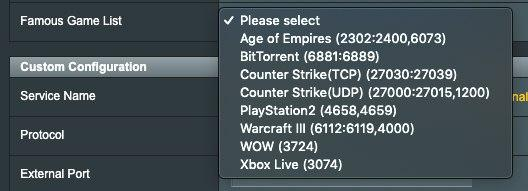
\includegraphics[width=.75\linewidth]{./assets/famous-games.jpg}
\caption*{A router's configuration screen, showing a list of "famous games" including Bittorrent. From \href{https://twitter.com/tjhorner}{@tjhorner} on Twitter.}
\end{figure}
\end{frame}

\begin{frame}[label={sec:org14fc2bd}]{Security vulnerabilities}
  \note{Clearly, there are lots of opportunities for the software we run on our
    routers to face security vulnerabilities. However, when we're picking out
    our stack ourselves, we have the option to limit our risk by choosing a
    minimal set of tools-and updating quickly, or as quickly as our vendor can.}

  \begin{itemize}
  \item Insecure default passwords and configurations
    \note{There are insecure default settings on so many routers, and they often
      support management protocols which are also inherently insecure.}

  \item<2->{Out-of-date protocol stacks}
    \begin{itemize}
      \item<3-> WPAv3
      \item<4-> TLS 1.3
      \item<5-> SHA-1 deprecation
        \note{
          We don't \emph{use} SHA-1 any more, but I can guarantee there's a lot of
          equipment out there that still uses it, or even requires it
          }
    \end{itemize}
    
  \item<6-> Vendor security vulnerabilities
    \begin{itemize}
    \item<7-> Netgear routerlogin.net private cert
      \note {
        \href{https://gist.github.com/nstarke/a611a19aab433555e91c656fe1f030a9}{Netgear's routerlogin.net private cert} was found to have been leaked \emph{while I
          was writing this talk} and that's far from the only security issue we've
        seen.}

    \item<8-> Cisco NX-OS CVE-2020-3119
      \note{Turns out, Cisco's NX-OS' management protocol has a \href{https://nvd.nist.gov/vuln/detail/CVE-2020-3119}{stack overflow
          vulnerability}, which, combined with the OS' weak ASLR, lack of stack
        canaries, and the privileged context of the CDP parser means that a
        successful attack is devastating.}
    \end{itemize}
  \end{itemize}
\end{frame}

\begin{frame}[label={sec:org3f5e855}]{Complex systems encounter complex failures}
\note{
    Above a certain complexity, systems encounter emergent behaviors: unexpected
    and undesigned-for modes of operation that can manifest as failures and
    errors in ways that you may not understand. Actually building some
    familiarity with how networks work at a low level can help you comprehend
    what's happening when your systems fail.}

  \begin{figure}[htbp]
    \centering
    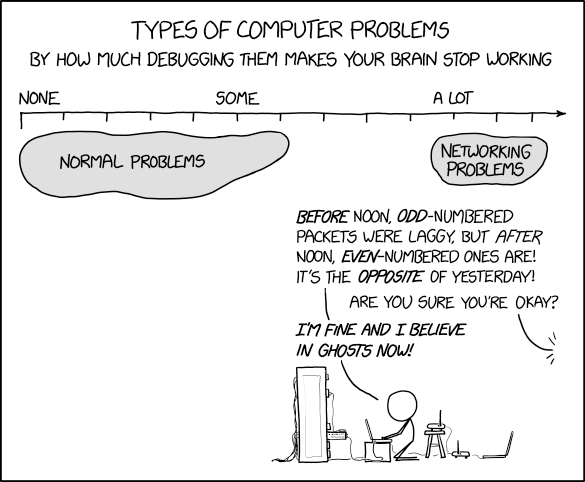
\includegraphics[height=.6\textheight]{./assets/networking_problems.png}
    \caption*{Take a bunch of complex systems and stick them together\ldots{} it'll be fine, right? (XKCD~\href{https://xkcd.com/2259}{2259}, ``Network Problems''. CC-BY-NC~2.5)}
  \end{figure}

\note{
    When building out a network, you're taking a bunch of complex systems, and
    by integrating all of them together, creating an even more complex
    meta-system. Debugging this system without context is difficult, to say the
    least, and you'll have more of a fighting chance with a deeper understanding
    of how a router actually operates-and what goes into network design.}
\end{frame}

\subsection{Goals for our router}
\label{sec:org778996d}

\frame{\subsectionpage}

\begin{frame}[label={sec:org8d79961}]{Be upgradeable}
  \begin{itemize}
  \item<2-> Have expansion ports
  \item<3-> Support future protocols and needs
  \item<4-> Avoid getting trapped with insufficient hardware
  \end{itemize}
\note{While inexpensive, consumer routers are often extremely limited; if you look
at the OpenWRT wiki, there's an entire warning about 4/32 devices, which
have only 4MB of RAM and 32MB of flash storage; these devices can barely fit
their firmware when they're shipped out, let alone run extra tools! By using
commodity desktop hardware, we can swap out components, such as adding
higher-bandwidth NICs (10GbE hardware is pretty inexpensive now) or other
specialized additions.}
\end{frame}

\begin{frame}[label={sec:org1c4cf14}]{Be easy to manage}
  \begin{itemize}
  \item<2-> Familiar network analysis tools
  \item<3-> Interfaces that we use routinely
  \item<4-> Your choice of package management
  \end{itemize}
\note{
Instead of trying to figure out what strange configuration is present, or
divine what IP address has gotten assigned, all of your familiar command
line tools, like or are there, close at
hand.}
\end{frame}

\begin{frame}[label={sec:org100ce9b}]{Be a test bed for exploring network ideas}
A full operating system on your router offers you lots of opportunities to
try out different tools or technologies

\begin{itemize}
  \item<2-> Docker containers on your router
    \note{I host my Unifi Controller on my router as a Docker container, which avoids
      using a separate physical device}

  \item<3-> Dynamic DNS
  \item<4-> A little home website
  \item<5-> Logging or traffic analysis
\end{itemize}
\end{frame}

\section{Selecting hardware}
\label{sec:org7a3497d}

\frame{\sectionpage}

\note{
  I'm starting with hardware selection, but really both hardware and software
  have to be considered in tandem, since one will inform the other. This may
  evolve as you build your system, too! Maybe you decide that one approach isn't
  working for you after you've done some basic setup. That's okay. Just remember
  to take notes and log your progress.}

\subsection{Constraints \& parameters}
\label{sec:org9880863}
\note{
  Obviously, what capabilities you want to focus on will define how you select
  hardware to some extent; the short form is that as you want to have more
  capabilities captured in your router, you'll need more resources in general;
  there are some areas where you can optimize for a specific function.}

\frame{\subsectionpage}

\begin{frame}[label={sec:org4c417ad}]{RAM}
  4GB of RAM is more than enough \ldots
  \vfill
  \onslide<2->
  \ldots but if you want to do exciting projects, you might want even 16 or 32.
  \note{4GB of RAM is more than enough for a basic firewall; if you want to add more
    services, however, you'll want more. Once you start considering
    virtualization, 16 or 32 might be needed or useful.}
\end{frame}

\begin{frame}[label={sec:org5a31146}]{CPU}
  You don't need a lot of power here; an Intel Atom is plenty for basic routing needs.

  \vspace{3ex}
  \onslide<2->
  I'd always recommend a multicore CPU, however.
\note{Any recent CPU will be powerful enough--here your concerns are cost and
heat, mainly. Low-power embedded CPUs are great for low- or no-noise
operation. I do recommend multi-core, and if you'll be doing more crypto
on-board (TLS termination, VPN endpoint) your CPU should have SIMD
instructions.}
\end{frame}

\begin{frame}[label={sec:org7599d13}]{Storage}
  \begin{itemize}
  \item<2-> Minimal amount needed to start - a flash drive will do
  \item<3-> Speed of storage is not a priority
  \item<4-> Extra capacity for bigger projects can be on a normal SATA HDD
  \end{itemize}
  \note{
    120GB SSDs are \$20 or less on Newegg; a lot of boards designed for a usecase
    like this are also built to be booted off of flash drives or SD cards.
    If you're interested in doing more edge computing on your router-logging,
    traffic shaping, running an HTTP server for a personal website (why not?)
    you might want additional storage. This doesn't need to be an SSD, spinning
    platters will do fine.
  }
\end{frame}

\begin{frame}[label={sec:orgfdc6a4f}]{NICs}
  \note{
    This is the heart of choosing what you'll use as a router; at a minimum, you
    need two interfaces: one external, one internal. If you've got a separate
    switch you're using for your internal network, that may be all you need; if
    you want other machines directly connected to your router, however, you'll
    need more.}
  \begin{itemize}
  \item<2-3> Onboard, on-motherboard NICs
    \note{
      Assuming your motherboard has at least two NICs, you can forego all of the
      complexity and just use those devices.}

  \item<3> PCIe card NIC
    \note{
      If you want to do a little more than the motherboard can support directly,
      either in capacity or speed (or both!) an add-in card might be a good
      choice. With a PCIe card, you can get SFP+ ports and full 10GbE speeds.

      One issue I've encountered is, if you install an expansion card NIC, some
      motherboard firmwares will disable the onboard NIC by default. You may want
      that! In my case, I really didn't. So, if your NIC suddenly doesn't work when
      you install an additional one, you should look for this in the BIOS/EFI.}
  \end{itemize}
\end{frame}

\begin{frame}{NIC caveats}

  \begin{itemize}
  \item<2-> Drivers a consideration
    \note{
      A key point with NIC selection is driver support; depending on your OS choice,
      you may be more or less limited here! I recommend picking your NIC in
      conjunction with your OS or after-so you can confirm what support you'll
      have.}
  \item<3-> Link Aggregation/Bonding and VLANs
    \note{
      You may encounter a situation where you want the core components of your
      network to be on one subnet, and to have client devices on another; if
      you've got a switch that can allocate ports to VLANs, then you can use one
      larger, more capable switch to handle multiple subnets in parallel-but that
      does require that your drivers support multiple VLANs on the same
      connection, otherwise you'll need a separate connection from the router for
      each subnet.}
  \item<4-> Initial capacity requirement
    \note{
      When choosing a NIC for your build, you should keep your throughput
      requirements in mind; if you host a media server inside your network, you
      may want to have higher throughput on your LAN connection than your
      WAN. Just try to keep your upstream and downstream in excess of what you'll
      need for your connection.}
  \item<5-> System I/O capacity for future upgrades
    \note{When you're looking to upgrade, or planning for future upgrades, make
      sure you have the physical capacity to install new devices.}
  \end{itemize}
\end{frame}

\subsection{Approaches}
\label{sec:org1558c43}

\frame{\subsectionpage}

\begin{frame}[label={sec:org3e08734}]{Pre-built}
\note{Often slightly more expensive, but featureful systems. When looking at
    prebuilt equipment that runs pfSense or other similar firewall-oriented
    operating systems, you'll see purpose-built, but closer to commodity
    hardware than if buying from a vendor who builds a custom router OS like
    Ubiquiti or MikroTik.}

  \begin{itemize}
  \item<2-> Netgate firewalls
    \note{Ship with a pfSense license, this is great if you want an integrated
      solution.}
  \item<3-> fitlet IoT Gateways
    \note{These are basically the minimal necessary component for a firewall.}
  \item<4-> QNAP
    \note{
      Mostly a NAS vendor, they have some switches and network equipment,
      including what they call a \href{https://www.qnap.com/en/product/qgd-1600p}{smart edge switch},
      which looks a lot like what we're describing here.}
  \end{itemize}
\end{frame}

\begin{frame}[label={sec:org1e54b71}]{Small Form Factor}
  \begin{itemize}
  \item<2-> Standard desktop box
    \note{Any relatively recent SFF desktop will do, as long as you can install
      the parts you want to use in it!}

  \item<3-> PCEngines APU units
    \note{Useful boards for custom installations; if you're very space
      constrained or have limited need for expandability, this might be a good
      choice.}
  \end{itemize}
\end{frame}

\begin{frame}[label={sec:org94796ed}]{Rackmount}
  Build your own
  \onslide<2>
  \begin{figure}[htbp]
    \centering
    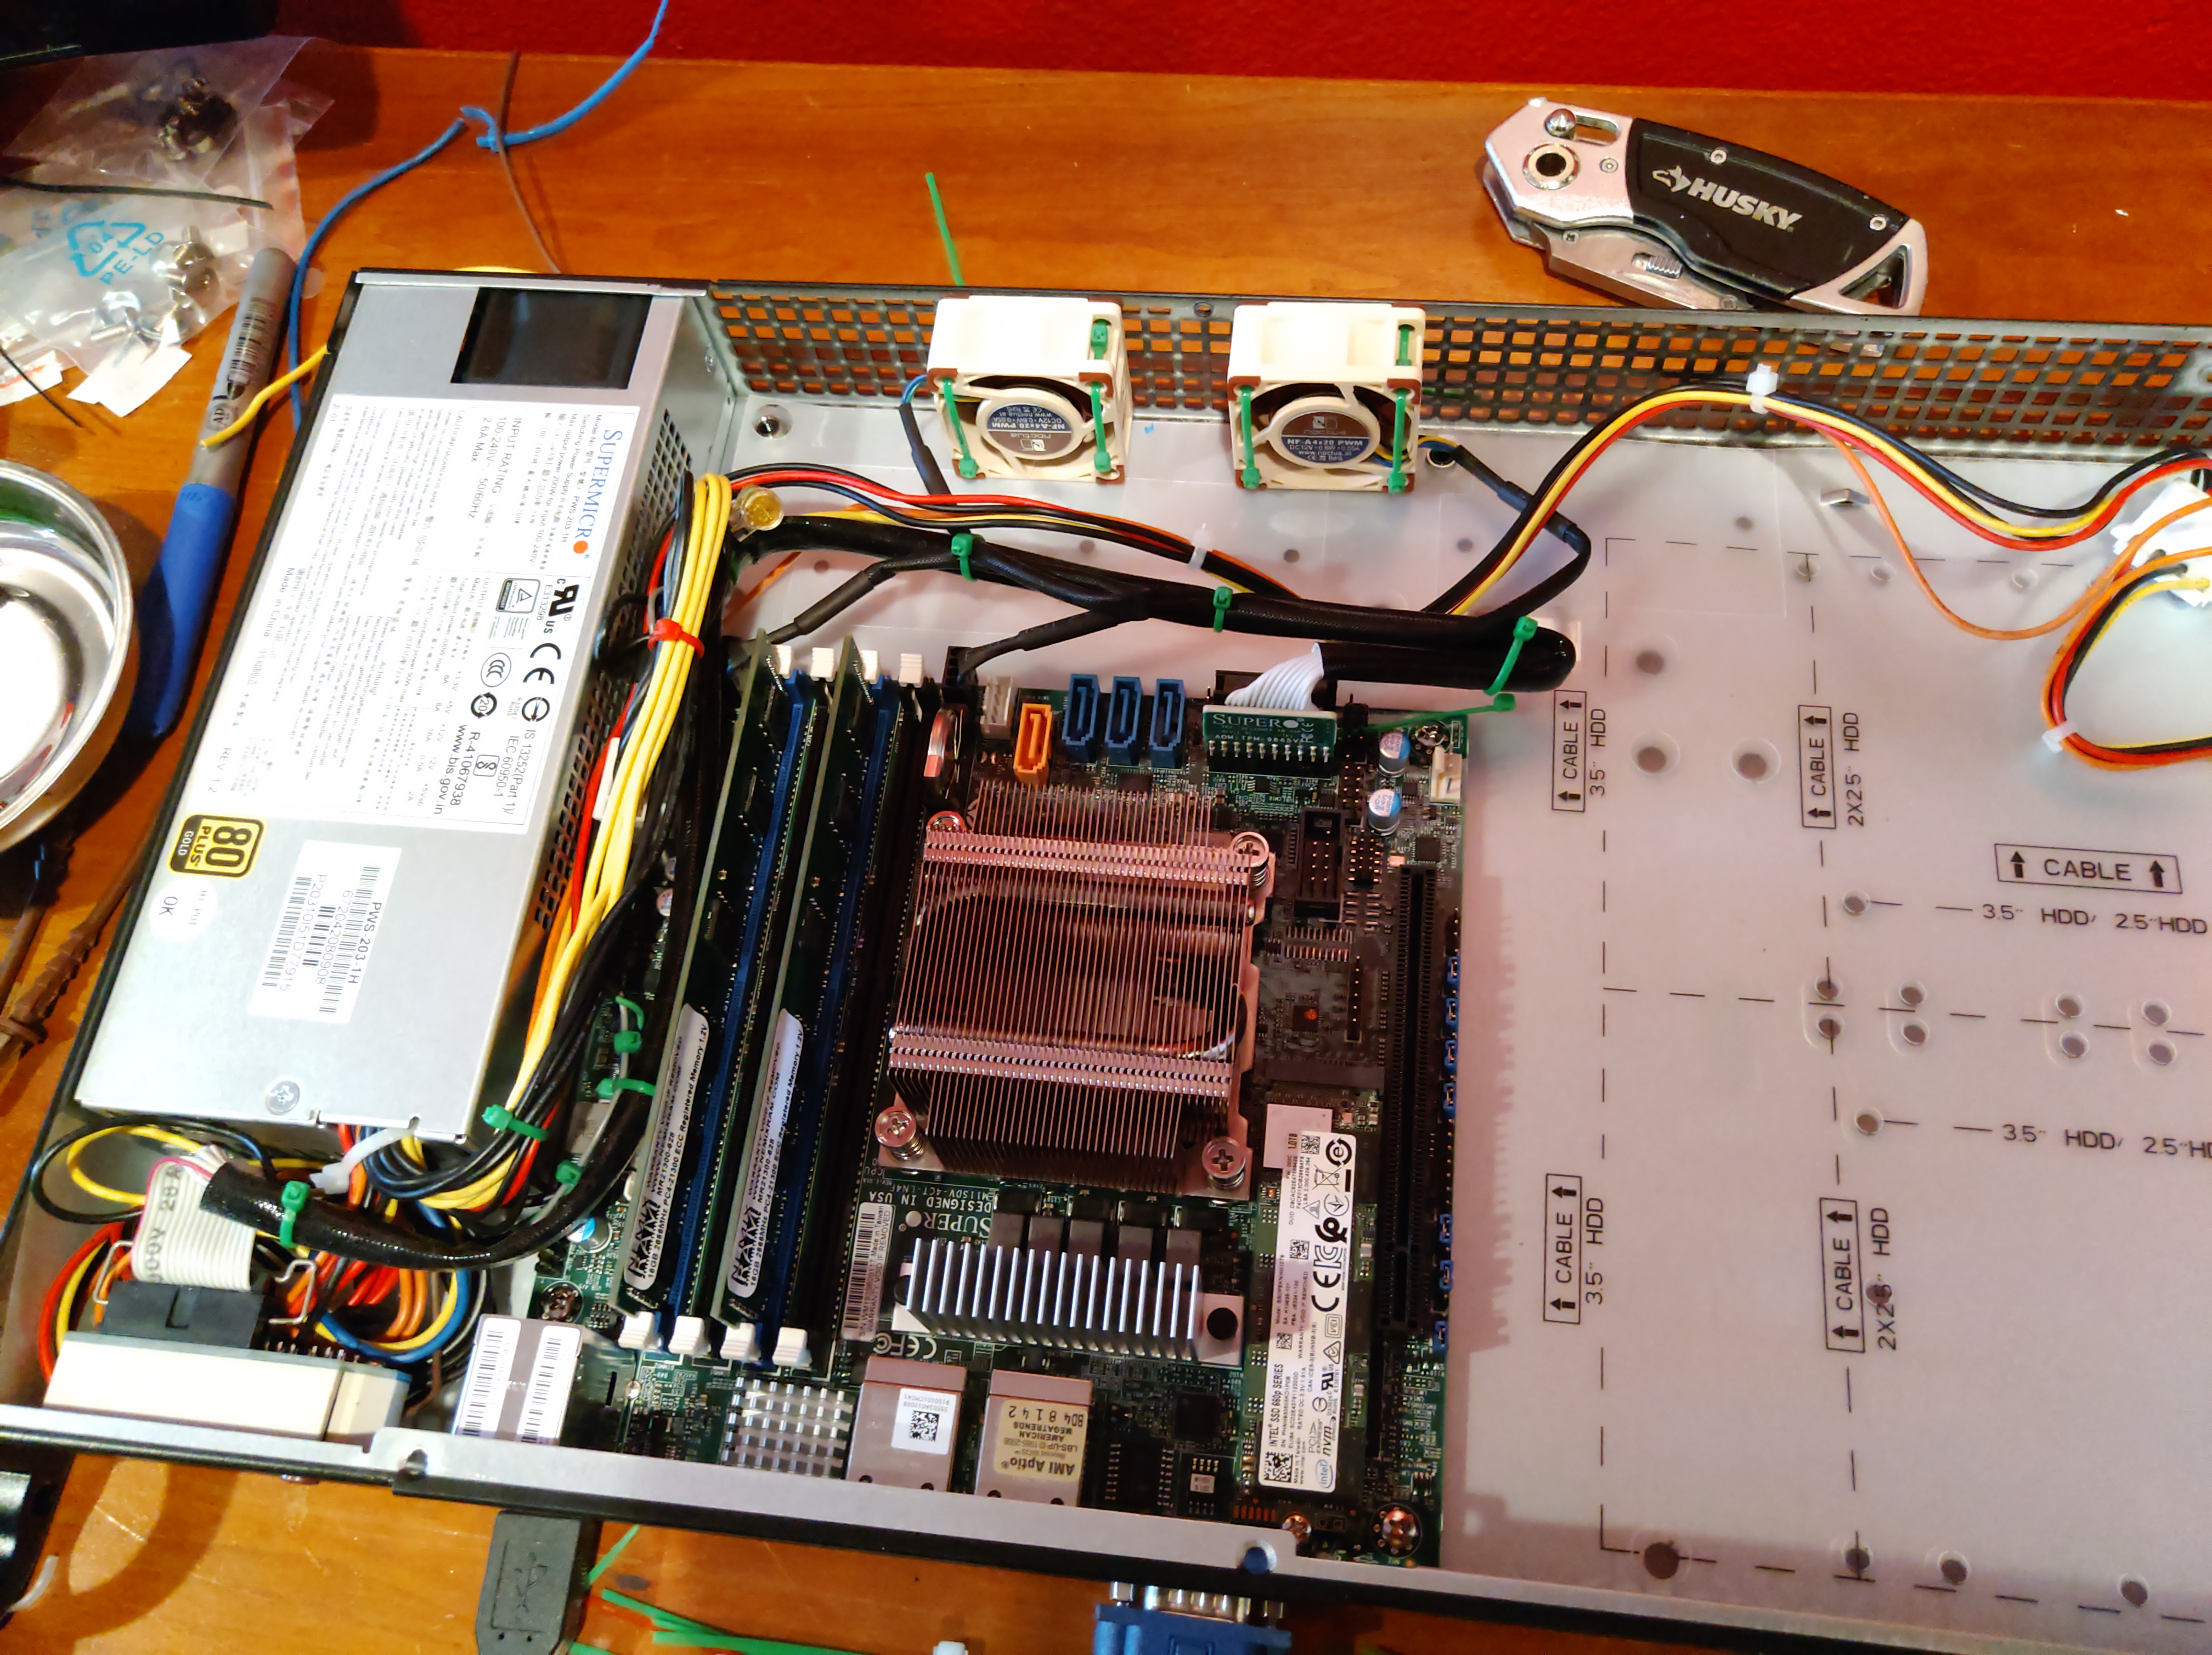
\includegraphics[height=.6\textheight]{./assets/router-cm.jpg}
    \caption*{A custom Supermicro build in a 1U switch-depth chassis}
  \end{figure}
  \note{Order parts from Supermicro, Tyan, other vendors, and build yourself
    a box! This is a more expensive route, but can be very rewarding. If
    you're building with Supermicro, do be aware that working in their cases
    can be a little like kitbashing, and might involve some initially
    questionable approaches. <Photos of my router build.>}
\end{frame}

\begin{frame}{Rackmount}
  \ldots or buy used!
    \note{
      There's plenty of 1U servers with fantastic loadouts available for
      relatively low prices. A manufacturer I was recently introduced to is HYVE,
      who have some really cute boxes; they've got a focus on warm-temp
      datacenters, and they're blue!}
    \onslide<2>
    \begin{figure}[htbp]
      \centering
      \includegraphics[height=.6\textheight]{./assets/duwamish-open.jpg}
      \caption*{A HYVE Zeus secondhand server}
    \end{figure}
\end{frame}

\subsection{Considerations for expandability}
\label{sec:org0ee9e3f}

\frame{\subsectionpage}

\begin{frame}[label={sec:org2c89497}]{Future network standards}
  \begin{itemize}
  \item<2-> Gigabit now, what next?
    \note{
      10 Gigabit hardware is getting really inexpensive! If you've got 8 PCIe gen 2
      lanes available, you can have a dual SFP+ card. If you've got more, you can do
      oh so much more. I've found multi-10-Gig/multi-gigabit cards, which can be handy
      for virtualization down the line.}

  \item<3-> Wireless upgrades
    \note{If you get a wireless card that can run in AP mode, you can use your router as
      your access point-and even trade out parts to upgrade to new standards as they
      become available.}
  \end{itemize}
\end{frame}

\begin{frame}[label={sec:orgfcacbf9}]{Additional different hardware}
  \begin{itemize}
  \item<2-> Tensorflow PCIe!
    \note{
      You can use Tensorflow in hardware now, relatively cheaply. They're \href{https://www.mouser.com/ProductDetail/Coral/G650-04527-01?qs=sGAEpiMZZMsG1k5vdNM\%252Fcyg9iDc\%25252Bz9JYkOSrS1TKoVU\%253D}{\$35 at
        Mouser.} What would I do with these? I have no idea yet! But if you wanted to use
      some tool like greylog to capture logs, you could run an ML model analysis on
      it, and do so more efficiently than just on your CPU.}

  \item<3-> TPM for security stuff
    \note{While TPM support is limited generally, you can use it as a source of HWRNG, and
      it can sometimes be used to offload cryptographic computations.}
  \item<4-> Cellular connection for reliability
    \note{mSATA cell modems can allow your router to have a failover connection
      in cases where your main network connection fails-due to a power outage,
      for instance.}
  \end{itemize}
\end{frame}

\section{Software stack}
\label{sec:org2fd137a}

\frame{\sectionpage}
\note{This is an area where there's lots of hot-headed opinions, and lots of options
  without significant distinction. Decide what matters to you from the axes I'll
  present, and remember that this choice is not permanent. You can try something,
  decide it doesn't work, and change it out! That's okay!}

\subsection{Axes of choice}
\label{sec:org84da425}

\frame{\subsectionpage}

\begin{frame}[label={sec:orgb205e75}]{Interface style}
  \note{
    Some options are more configurable through webpages and graphical
    environments, but are less configurable through text interfaces; careful
    configuration of interfaces and potentially a VPN may be needed to remotely
    manage some of these stacks.

    For a more complete list to explore, check out \href{https://en.wikipedia.org/wiki/List\_of\_router\_and\_firewall\_distributions}{the list on Wikipedia}.}

  \begin{itemize}
  \item<2-> Graphical/Web
    \begin{itemize}
    \item pfSense
    \item OPNsense
    \item \href{https://www.clearos.com/}{clearOS}
    \item \href{https://zeroshell.org/}{zeroshell}
    \end{itemize}

  \item<3-> Textual
    \begin{itemize}
    \item firewall-cmd (on any distro that supports it)
    \item shorewall
    \item \href{https://www.vyos.io/}{VyOS} - both free and paid, this one's complicated. Derivative of Brocade
      Networks' OS.
    \item Raw nftables on any recent Linux version
    \end{itemize}
  \end{itemize}
\end{frame}

\begin{frame}[label={sec:orgdb902ba}]{Preference in base OS}
The mon0wall derivatives (pfSense, OPNsense) are all FreeBSD derivatives; in
other cases, you may prefer running a Linux kernel-for familiarity's sake,
or because of hardware support.
\end{frame}

\begin{frame}[label={sec:org991cbe7}]{Support model}
  \begin{itemize}
  \item Community-only
  \item Community version with paid extension
  \item Paid-only
  \end{itemize}
  \note{Paid support options exist for many firewall-oriented distros and
    derivatives; generally speaking, there's also community support available,
    but you may or may not find what you need in forums, especially when dealing
    with unusual hardware or network configurations.}
\end{frame}

\section{Configuring a router}
\label{sec:org2055775}
\frame{\sectionpage}

\begin{frame}
  So, we have the parts, how do we set it up?
\end{frame}
\note{
  For our demo here, I'm going to use Fedora, and I'm going to configure it with
  very low-level tools, to highlight fine details that graphical environments
  might gloss over.}

\subsection{Installing the OS}
\label{sec:orgfdf5a5f}
\begin{frame}{State should be self-maintaining}
  \note{There's lots of approaches to designing a system, and for a hobby server
    some of this overhead may be unnecessary, but it's a good habit to get into,
    and I've often found that having a philosophy in mind about how you're going
    to configure a system leads to a cleaner design.}
  \begin{itemize}
  \item<2-> System configuration should be automatic
    \note{For a reliable and lower-stress administration experience, configure
      components-firewall, services, applications-to start automatically and
      self-configure themselves.}
  \item<2-> Reboot often to test your configuration
    \note{After installing a new component and configuring it, save your
      configuration, then reboot to confirm that the component is actually
      waking when it's needed.}
  \item<3-> High uptimes don't equate to reliability
    \note{A machine that hasn't been rebooted since a major update is in an
      unconfirmed state, and that's an unsafe machine.}
  \item<4-> Lots of tooling isn't necessary for a one-off build
    \note{I won't cover Ansible or orchestration here, but if you're creating
      more than one system, you may want to take the configuration you've built
      and use automation to make it repeatable!}
  \end{itemize}
\end{frame}
\note{
  This part is probably the most ordinary aspect of this build. I'm going to use
  Fedora Server, and I'm going to leave any graphical components out, while
  making sure to set up SSH from the beginning.}

\begin{frame}[fragile,label={sec:org98c7403}]{Important software to install before starting your journey}
  \note{Before we start configuring components, it's a good idea to have a few tools
    quick at hand. I like all of my machines to have the basic tools for monitoring}
  Set up some basic tools to simplify your configuration process. I've chosen a few examples to use:
  \begin{itemize}
  \item<2-> Text editor: \texttt{nano}
    \note{
      I'm not normally a nano user, but it's got a very straightforward interface, and
      all I really care about here is being able to edit files on the machine. I don't
      care about having the most ergonomic environment for my daily driver needs.}

  \item<3-> Terminal multiplexer: \texttt{tmux}
    \note{Again, you may prefer other tools, but this is one I'm generally comfortable
      with, and can usually get around in easily. If you're going to remote into your
      machine a lot, you may want to configure it to be comfortable for you--but that
      is not the goal of this exercise.}
  \item<4-> System hardware monitoring: \texttt{ipmitool}
    \note{For a VM, this isn't so necessary, but on a server with onboard IPMI,
      it's nice to be able to see what the system's reading out. I routinely use
      \texttt{watch ipmitool sensors} in a \texttt{tmux} window.}
  \end{itemize}
\end{frame}

\subsection{Configuring routing}
\label{sec:org5b3a27e}

\begin{frame}[label={sec:org8d7dd3d}]{Choose your network configuration tool}
  \begin{itemize}
  \item<2-> systemd-networkd
  \item<3-> NetworkManager
  \item<4-> netplan
  \end{itemize}
  \note{NetworkManager, systemd-networkd are both viable options; here I'm using
    systemd-networkd since it's what I've been using at home.}
\end{frame}

\begin{frame}{Interface-specific configuration}
  Different aspects of our network configuration will go through different areas:
  \begin{itemize}
  \item<2-> \texttt{/etc/sysctl.d} files for interface-specific settings
  \item<3-> Network configuration depending on your management mechanism
    \begin{itemize}
    \item<4-> \texttt{/etc/NetworkManager/NetworkManager.conf}
    \item<5-> \texttt{/etc/systemd/network} files
    \end{itemize}
  \end{itemize}
\end{frame}

\note{Configuration files will be applied in alphanumerical order, and later
configurations will override earlier ones; it's reasonable to have
baselines defined in low-numbered scripts, and more custom configurations
in high-numbered scripts. All network setups do this.}

\begin{frame}{NetworkManager config}
  NetworkManager 

\begin{block}{Static or dynamic IP allocation}
\begin{block}{Static IP}
Useful for your gateway address on internal networks, or if you have a
static IP allocation from your ISP.
\end{block}

\begin{block}{Dynamic IP}
Handy when your upstream address is provided by DHCP; less handy if you're
trying to have routes declared statically.
\end{block}
\end{block}
\end{frame}

\begin{frame}[label={sec:org3a006ff}]{Multiple subnets and restricted routing}
  \begin{itemize}
  \item<2-> Non-routing subnet (\texttt{net.ipv4.conf.\$IFACE.forwarding = 0})
    \begin{itemize}
    \item<3-> Keep IoT devices off the wider internet
    \item<4-> Securely access IP cameras
    \item<5-> Examine untrusted devices?
    \end{itemize}
  \item<6-> Egress-only subnet
    \begin{itemize}
    \item<7-> Can reach the broader internet
    \item<8-> Can't see other local subnets
    \item<9-> Great for devices that need to phone home, but that you don't trust
    \end{itemize}
  \end{itemize}
  \note{One useful configuration is to deliberately block IP forwarding on an
    interface, to restrict the potential for devices (IoT in particular) to
    leak information you might not want visible on the broader network. In this
    case, you'd still run DHCP on the interface, but you would not present a
    route to that network, and you would deliberately block forwarding for that
    NIC.

    Normally, to collect information from IoT devices that aren't routing to
    the broader network, you need a dual-homed machine to collect logs or video
    streams, for instance; when you're running a full Linux install on your
    router, it \emph{is} a dual-homed machine, and can provide the access you
    need. If you want to do more to limit your firewall's exposure, you might
    consider a virtual machine; we'll talk about that in \ref{sec:org8517efe}.

    To allow devices to only connect to the broader internet, you'll allow them
    to forward packets, but use a firewall rule to drop packets intended for
    other local subnets.
  }
\end{frame}

%% \subsection{Configuring IPv6 routing (Optional)}
%% \label{sec:orgab512e8}
%% \begin{frame}
%%   So what's that IPv6 thing about?
%% \end{frame}

%% \begin{frame}[fragile,label={sec:orgf2a58cf}]{SLAAC and PD-assigned address}
%%  \begin{block}{\texttt{accept\_ra} and the tri-state boolean}
%% From \href{https://www.kernel.org/doc/Documentation/networking/ip-sysctl.txt}{\texttt{ip-sysctl.txt}} in the Linux kernel documentation,
%% \begin{quote}
%% Possible values are:
%%     0 Do not accept Router Advertisements.
%%     1 Accept Router Advertisements if forwarding is disabled.
%%     2 Overrule forwarding behaviour. Accept Router Advertisements
%%       even if forwarding is enabled.
%% \end{quote}

%% Note that this means we'll want to set \texttt{accept\_ra} to \texttt{2} \emph{specifically} on our
%% WAN interface for IPv6 support.
%% \end{block}
%% \end{frame}

%% \begin{frame}[label={sec:orga4304bc}]{6to4 tunnel (Hurricane Electric)}
%% \end{frame}

\subsection{Configuring firewall rules}
\label{sec:org19a3785}

\begin{frame}[fragile,label={sec:org1530f3c}]{nftables versus frontends}
  \begin{itemize}
  \item<2-> Not really a ``versus'' situation
  \item<3-> Pick your frontend, or just write scripts
  \item<4-> For the demo, we'll use \texttt{firewalld}
  \end{itemize}
  \note{Not really a "versus" here, but configuring nftables directly instead of using a
    frontend is a viable path, and if you have custom logic for null-routing
    specific IPs, you might want to have your own custom tooling writing your \texttt{.nft}
    files and applying them. For this talk, we'll use firewalld. It's close to the
    same syntax, but has some nice-to-have details like port numbers having service
    names.}
\end{frame}

\begin{frame}[label={sec:org9196245}]{Don't block ICMPv6!}
  \note{Coming from an IPv4 background, you might be tempted to try blocking
    ICMPv6 on your network out of an abundance of caution, reasoning that
    otherwise an attacker could map your network space.

    Given that the smallest subnet an ISP will issue is a /64, there's no reason
    to worry about your IP space being mapped, and ICMPv6 is used for so much!}
  (Short digression into IPv6 here.)
  
  ICMPv6 does a lot of heavy lifting in the IPv6 world! Here's a few things it
  does:
  \begin{itemize}
  \item<2-> Router solicitation and advertisement (replaces DHCP)
  \item<3-> MTU discovery
  \item<4-> Neighbor solicitation and advertisement
  \end{itemize}
  
  \note{It's hard to stress this enough. Blocking ICMPv6 is a great way to cause
    arbitrary, difficult-to-diagnose slowdowns if you have IPv6 support
    enabled. This isn't going to improve your security posture, SLAAC with
    security extensions will handle that.}
\end{frame}

\begin{frame}[label={sec:org87a247f}]{Forwarding and NAT}
\end{frame}

\subsection{External services}
\label{sec:org55a4d52}
\begin{frame}{Running extra services}
  You have a server at your disposal, make use of it!

  You can make your router accessible and functional when you're at home, and away.
\note{Part of the fun of running your own firewall is being able to host services on
it that would be limited or impossible on consumer hardware, and might be
difficult to configure on commercial hardware. Some of these can be quality of
life improvements (and may even be relatively straightforward to configure,
as some of them would need to exist inside your network as well.)}
\end{frame}

\begin{frame}[fragile,label={sec:org8635474}]{SSH}
  
 Being able to remotely connect to your firewall and check on the state of your
 local network is useful--especially if you're away from home, and want to make
 sure that a service is working. However, you'll want to take some precautions.

 \begin{itemize}
 \item<2-> Before enabling access on your WAN interface
   \begin{itemize}
   \item<3-> Add a key to \texttt{authorized\_keys}
   \item<4-> Disable password auth
     \note{
       Add at least one public key to your user's authorized\_keys, validate that
       you can connect with that key, then disable password authentication. Best
       practices for SSH keys include using a different one on each device that
       needs to connect, and potentially using a different key for each service
       that you connect to with them. I recommend using \href{https://en.wikipedia.org/wiki/EdDSA\#Ed25519}{Ed25519} as the cipher;
       it's short and powerful.}
   \item <5-> Disable root login
     \note{Most linux installs do this by default now, but it's always good to
       check.}
   \end{itemize}
 \item<6-> When enabling on your WAN interface
   \begin{itemize}
   \item<7-> Optionally, use a nonstandard port
     \note{This is optional, but reduces the number of random drive-by attempts that
       you'll see. I'm a fan of port 24. This can be done just with a firewall
       rule, even!}

   \item<8-> Consider fail2ban, logging
     \note{In cases where you look at your \texttt{journalctl} logs and see lots of
       attempted connections, you might consider adding fail2ban, and setting
       some sufficiently high threshold--10 attempts, maybe. Remember when doing
       this that it can bite \emph{you}, too.}
   \end{itemize}
 \end{itemize}
\end{frame}

\begin{frame}[label={sec:org79d4237}]{Nice-to-have services}
  \begin{block}{VPN}<2->
    \note {Here we get into nice-to-have functionality, beyond the absolutely necessary. If
      you want direct access to hosts inside your network from a remote location,
      you'll want to use a VPN.

      There's several approaches to this, largely depending on how willing you are to
      DIY parts of the solution. Helpfully, \href{https://git.kernel.org/pub/scm/linux/kernel/git/torvalds/linux.git/commit/?id=bd2463ac7d7ec51d432f23bf0e893fb371a908cd}{Torvalds merged Wireguard into his branch
        for 5.6}, so we should be able to rely on that being in production kernels soon,
      and you won't need to install separate modules to get it working. There's a few
      frontends for Wireguard under development now, but if you don't want to use
      those there's OpenVPN, which is significantly more mature.}
    \begin{description}
    \item<3-> [OpenVPN] Well-known, broadly supported with clients for most platforms.
    \item<4-> [Wireguard] Recently integrated into the next kernel release, a faster
      but less broadly supported option.
    \end{description}
  \end{block}

  \begin{block}{Dynamic DNS}<5->
    \note{
      Instead of memorizing your IP address, why not use a domain name? Services like
      no-ip can offer you a way to get back to your own machines relatively easily,
      but if you're willing to pay a little for a domain, there are plenty that are
      very cheap--and then you just need to set up a script to auto-update your DNS
      record regularly. Personally, I like Hurricane Electric for my DNS hosting
      needs, but there's lots of options out there. Pick one you like, and have fun!}
    \begin{itemize}
    \item<6-> no-ip or similar for quick access
    \item<7-> Get a domain name and use a nameserver with a DDNS API, and use a script to update
    \end{itemize}
  \end{block}

  \begin{block}{Personal webpage}<8->
    \note{
      Once you've got a domain name, clearly you need a website, too. Consider getting
      a Let's Encrypt cert, while you're at it! Note that this is a fantastic service
      to run in a container, or on another machine with port forwarding. If you take
      the port forwarding route, just make sure to enable forwarding for as many ports
      as you'll end up using--often both 80 and 443 are sufficient.}
    If you set up a domain name, consider hosting a webpage with a simple server
    \end{block}
\end{frame}

\subsection{Debugging}
\label{sec:orgedb5cb4}

\begin{frame}
  Something went wrong!

  What to do?
\end{frame}

\begin{frame}[fragile,label={sec:orgba55011}]{Tools}
  \note{All the tools you'd normally use to diagnose network connection issues
    apply-layer 3 and above tools to determine inter-network connectivity like
    \texttt{traceroute} and \texttt{ping}, but now we're also looking to understand firewall
    issues like if DNS requests are being blocked, or even some layer 2 issues, like
    whether or not our router's seeing ARP requests. This is where we start caring
    about the difference between received packets and processed packets, and where
    tools that interact directly with the NIC come in.}

  \texttt{ping} and \texttt{traceroute} or \texttt{dig} are invaluable, as is
  understanding the output of the \texttt{ip} family of commands; those are the
  same as a desktop, however.
 
  Some tools outside of the normal desktop network toolkit:
  \begin{description}
  \item[{tcpdump}] Collect logs directly from the firewall, on a given interface
  \item[{Wireshark}] Collect and examine \emph{pcaps}, packet captures. Lets you
    investigate failures at your leisure, and sift through captures
  \end{description}

  \note{If these tools don't work on your router, you have a NIC that doesn't support
    promiscuous mode (can pass through all packets, not just those for its MAC
    address)-most should, but it's possible some won't. In that situation, you'll
    need to find a different NIC to use if you want to be able to debug with these
    tools.}
\end{frame}

\begin{frame}[label={sec:org477961b}]{Classes of failure}
  \begin{itemize}
    \item<2-> Physical
      \note{Sometimes cables go bad. Sometimes NICs are bad. When a NIC's bad, one often has
        few options for recourse, but generally only a cable is bad. This might be as
        trivial as one of the conductors failing, or it may be as strange as a cable
        that's fine unless a specific frame goes through it. Bin the cable. Life's too
        short for bad cables.}

    \item<3-> Logical
      \begin{itemize}
        \item<4-> Configuration error
          \note{There's a great early-internet meme of the 500 mile email. Configuration
            errors can happen to the best of us, and they will manifest in myriad
            ways. Strange traffic patterns, machines that can't communicate with each
            other, things which work outside the network not working inside\ldots{} you
            name it!}

          \item<5-> Assumption fault
            \note{This is a fun one. Sometimes your logical error is not in software-it's in
              how you think about the situation. An assumption fault can come up all
              sorts of ways-routes that don't work, network segments not being
              shared-but when they're encountered, diagramming them can help.}
      \end{itemize}
  \end{itemize}
\end{frame}

\subsection{Recovery and fault-tolerance}
\label{sec:orgcb67d08}

\begin{frame}{Recovery and fault-tolerance}
    Failures happen, unfortunately. Power outages strike, hard drives crash,
    stray voltage kills your SSD's controller\ldots{}

    \ldots{} and then you need to get into your router.
\end{frame}

\begin{frame}[label={sec:orgbfa871a}]{Backups!}
  These can come in various flavors:
  \begin{itemize}
  \item<2-> Full-system disk images
  \item<3-> Configurations in a private (or public if that's your thing) repo
  \item<4-> Build log with detailed notes
  \end{itemize}
  \note{Backing up key information matters a lot; this can be in the form of a
    full-system backup, or as a build and design log. I'm a big fan of logging
    my builds in markdown, or Org mode, or whatever journalling mechanism is
    most convenient-then storing it in Git and keeping it off-site, on a service
    like Gitlab, Bitbucket, or Gitlab.}
\end{frame}

\begin{frame}[label={sec:org48c7f73}]{Break glass}
Maybe your only laptop with an SSH key for your router on it had a hard
drive failure, or you had a device stolen. In this case, if you can't get
into your router because you've properly locked it down, you're in a
pickle.

\begin{itemize}
\item<2-> IPMI or Serial Console access
  \note{Assuming you have physical access to the server, you can connect a serial
    console, and, assuming you've enabled it ahead of time for the machine, you
    can sign in directly through that interface. If you have IPMI that supports
    integrated KVM, such as a Supermicro machine or a suitably-licensed Dell or
    HP board, you can do the same direct login.}

\item<3-> Spare private key
  \note{
    Whether the private key is stashed in a password manager, on a USB stick,
    or encoded in a QR code, having an extra public key provisioned on your
    router, with the private key on a separate physical device allows you to
    maintain access to the router, from any device with an SSH client, without
    pre-provisioning it.

    With this mechanism, especially if the key is stored in some sort of
    off-site backup, you'll want to regenerate your break-glass key after
    resolving your lack of access, and stash the new one in its place;
    otherwise, your extra credential is now just another credential that you
    can use from that or any machine.}
\end{itemize}
\end{frame}

\section{Other configurations}
\label{sec:org319584b}

\begin{frame}{Other ideas}
  So, what else can we do?
\end{frame}

\subsection{Virtualized firewall}
\label{sec:org8517efe}

\begin{frame}{Other ideas}
  Virtualize it!
\end{frame}

\begin{frame}[label={sec:org10a5a15}]{Why virtualize?}
  \begin{itemize}
  \item<2-> Reducing risk from compromise
    \note{
      Being the gateway device that has the most internet-facing surface area, your
      firewall is a prime target for attack. By running the firewall as a virtual
      machine instead of as the host, you can apply more restrictions to the
      firewall than you could with it running as the main OS. Now, it can only
      access storage or any other device that is assigned to it.
    }

  \item<3-> Virtual firewall for virtual machines
    \note{
      A common approach to securing multiple virtual services is to run a
      firewall VM and have it act as the gateway for all of your virtual
      machines, instead of having the host also operate as the gateway; this
      approach allows you to have hidden services inside the network you've
      created, and treat your virtual network as you would a physical
      network.
    }

  \item<4-> Quick update/deployment
    \note{
      Updates to a virtual machine, depending on the approach, can be applied
      extremely quickly and with little downtime.}
  \end{itemize}
\end{frame}

\begin{frame}[fragile,label={sec:org80a262d}]{How to virtualize?}
  \begin{itemize}
  \item<2-> Pick your OS
    \note{
      Basically all the questions we asked above apply twice, now; we need to
      determine how much physical RAM our VM host needs, and of that amount, how much
      the VM needs. A multi-core processor, and preferably with a lot of cores, is
      essential.}

  \item<3-> Connect your VM to the network
    \begin{itemize}
    \item<4-> Linux Bridge interface
      \note{
        One option is to make your host also route packets, although this might be said
        to defeat the purpose of the firewall here.}

    \item<5-> \href{https://en.wikipedia.org/wiki/Promiscuous\_mode}{Promiscuous Mode NIC}
      \note{
        In this mode the NIC passes all packets it receives to the kernel, which means
        it can respond to multiple MAC addresses if the host(s) so choose; this is a
        common approach to allow one or multiple VMs to share a network connection with
        a host.}

    \item<6-> PCIe Passthrough NIC
      \note{
        For my virtual firewall setup, i've opted to dedicate an entire physical card
        with multiple ports to the firewall, and thereby made my VM host indirectly
        connected to the main network. To achieve this I ended up adding an instruction
        to load \texttt{pcistub} as the driver for a specific device to the kernel command
        line.}
    \end{itemize}
  \end{itemize}
\end{frame}

\begin{frame}[fragile,label={sec:org44af7c6}]{Issues you might run into}
  \begin{itemize}
  \item<2-> Drivers and PCIe Passthrough
    \note{
      I've been setting up an OPNsense VM to operate as the firewall for my
      hackerspace; the server I purchased to function as our new firewall is far
      more powerful than is necessary for a firewall alone, so I figured I'd host
      some extra machines alongside the firewall, and get more use out of the
      server.

      Well, the Chelsio NIC I added to the server required a fair amount of
      massaging to let me actually do the passthrough; I ended up needing to
      use the \texttt{pcistub} kernel command line option for the whole card to stop the
      kernel from loading the drivers for it.}

  \item<3-> Virtual bridged network
    \note{
      If you're using \texttt{virsh} to establish your networks, for a virtual network where
      the firewall VM is the gateway, you'll need to specify how all your VMs attach
      to it by configuring the network in their XML config to not have a forwarding
      entry.}
  \end{itemize}
\end{frame}

\begin{frame}{Other ideas}
  Have a firewall behind a firewall
\end{frame}

\begin{frame}{Multiple firewalls}
  \begin{itemize}
  \item<2-> Keep internet-accessible devices separated from ``soft hosts''
  \item<3-> DMZ is now outside of a firewall
  \end{itemize}
  \note{Seen as a "defense in depth" strategy, this takes the medieval walled city
  approach to network design. Here, we have potentially two levels of network;
  we might want to keep "soft hosts"--personal computers, other relatively
  unsecured systems--behind a more restricted firewall, while still allowing
  machines operating as servers to have a more porous environment to work
  in--potentially with other untrusted devices there as well (such as IoT
  devices).}
\end{frame}

\subsection{Tuning and speed improvements}
\label{sec:orgb9c111a}
\begin{frame}{Tuning for speed}
    \centering
    
\includegraphics[height=0.75\textheight]{./assets/packet-pinball.png}
    
    \raggedleft
    \small
    \href{http://deathgenerator.com}{Death Generator} by \href{https://twitter.com/foone}{@foone}
\end{frame}

\begin{frame}[label={sec:org13ce3d4}]{Jumbo Frames}
  When looking particularly at speeds above gigabit, you might notice that
  you're not getting as close to the ripping-fast speeds you expected.
  \vspace{3ex}

  Your throughput might look \textit{okay}, but not stellar.
\end{frame}

\begin{frame}{Jumbo Frames}
  Ethernet has some fixed overhead per-packet:
  \begin{itemize}
  \item Preamble: 7 octets
  \item Delimiter: 1 octet
  \item Destination MAC address: 6 octets
  \item Source MAC address: 6 octets
  \item 802.1Q header: 2 octets (Optional!)
  \item Length: 2 octets
  \item Frame check sequence (CRC32): 4 octets
  \item Inter-packet gap: 12 octets
  \end{itemize}
  That's 38-40 bytes per frame of overhead, just in layer 2.
\end{frame}
\note{
  By massively increasing the payload in an ethernet frame, since each frame's overhead is a fixed amount, for the same
  payload size you're sending 1/6 as many Ethernet headers.
  Ethernet frame overhead: 22B
  Standard MTU: 1500B
  IPv4 headers: $\geq$20B
  Overhead for an IPv4 packet in a standard ethernet frame: 2.8\% minimum
  IPv6 headers: $\geq$40B,
  Overhead for an IPv6 packet in a standard ethernet frame: 4.1\% minimum

  With jumbo MTU: 9000B
  IPv4 total overhead: 0.5\%
  IPv6 total overhead: 0.7\%

  This matters more for above-gigabit speeds, but where configurable jumbo frames can provide significant throughput improvements.

    The standard MTU is 1500B; this is fine in a reasonably fast network, but does
    have a not-insignificant amount of overhead. That MTU includes the IP header,
    after all, and especially on an IPv6 network, that can be quite large.

    There's unfortunately issues with using DHCP to announce the MTU of a network;
    many DHCP clients will simply ignore your stated value and use 1500, so until
    jumbo frames in consumer OSes start showing up more often, we're going to have
    to set this aside.}

\begin{frame}{Jumbo Frames}
  But Layer 3 gives us some overhead too.
  \begin{itemize}
  \item<2-> IPv4 headers: $\geq$20 octets
  \item<3-> IPv6 headers: $\geq$40 octets
  \end{itemize}
\end{frame}

\begin{frame}{Jumbo Frames}
  \begin{itemize}
  \item 1500 octet MTU overheads:
    \begin{itemize}
    \item IPv4: 1480 octet payload, 3.77\% overhead
    \item IPv6: 1460 octet payload, 5.07\% overhead
    \end{itemize}
  \item 9000 octet MTU overheads:
    \begin{itemize}
    \item IPv4: 8980 octet payload, 0.64\% overhead
    \item IPv6: 8960 octet payload, 0.86\% overhead
    \end{itemize}
  \end{itemize}
\end{frame}

\begin{frame}[label={sec:orgc8262cc}]{TCP offload}
An interesting technology but not widely supported; the primary vendor who's
pushing for this tech is Chelsio; they've \href{https://lwn.net/Articles/148697/}{attempted in the past} to get offload
support built into the Linux kernel, but were rebuked on the grounds that this
moves kernel decisions into a black box; we may yet see some changes in this
attitude, but it is generally outside the scope of this talk.
\end{frame}

\section{Lab}
\label{sec:org475924a}
\begin{frame}{Demo: Build a virtual router}
  
Let's build a router real quick!

Set up a virtual firewall for other virtual hosts (mayyybe?)

For the purposes of this section, we'll focus on a minimal firewall setup that
covers the basic needs of a firewall, with clear extension points.
\end{frame}

\subsection{Installing the OS}
\label{sec:org4390e2a}

\subsection{Setting up network configurations}
\label{sec:orgc20c062}

\begin{frame}{Setting up our virtual LAN}
  \begin{columns}
    \begin{column}{.45\textwidth}
      \vfill
      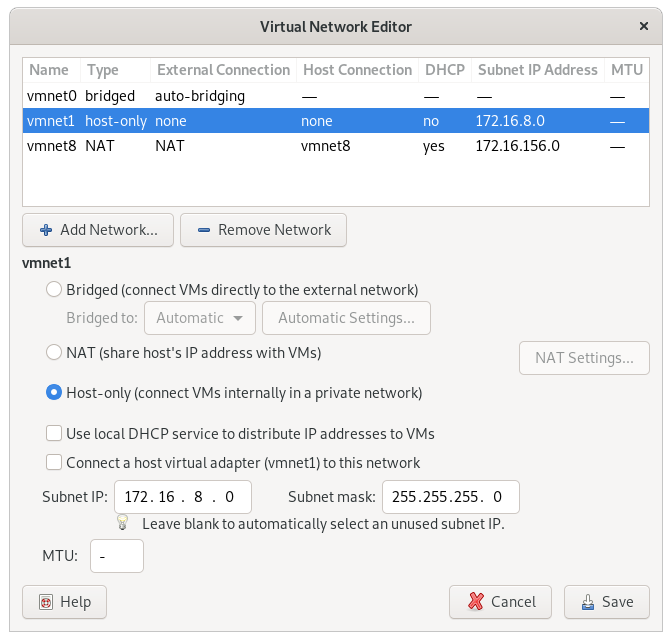
\includegraphics[width=\linewidth]{./assets/vnet-config.png}
      \vfill
    \end{column}
    \begin{column}{.45\textwidth}
      \vfill
      In VMware Workstation, you'll want to make sure that you have a host-only network
      where you've disabled DHCP and removed the host connection; we'll make this the
      private network managed by our firewall.
      \vfill
    \end{column}
  \end{columns}
\end{frame}

\begin{frame}{Setting up our virtual LAN}
  \begin{columns}
    \begin{column}{.45\textwidth}
      \vfill
      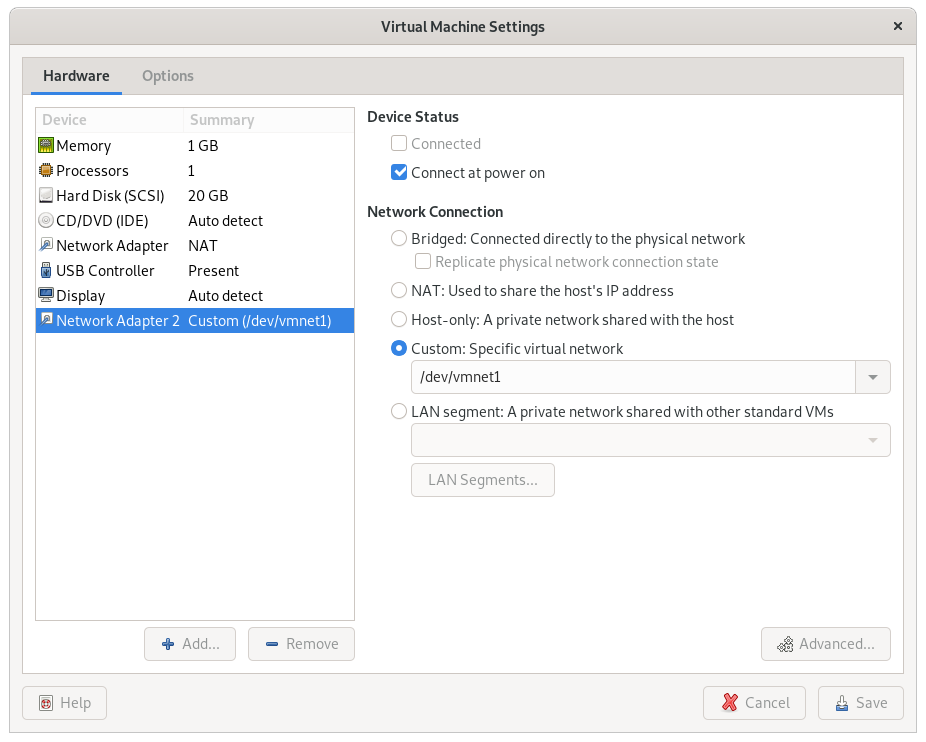
\includegraphics[width=\linewidth]{./assets/router-vm-network-settings.png}
      \vfill
    \end{column}
    \begin{column}{.45\textwidth}
      \vfill
      We'll also want to make sure to add this new network to our firewall VM.

      Any VMs created to use this network need to be configured to not have any
      other network connection.
      \vfill
    \end{column}
  \end{columns}
\end{frame}

\begin{frame}{Setting static IP}
  \note{Here we're creating a connection in NetworkManager on the ens36
    interface, with an address of 192.168.10.1. For this connection, we won't
    define a gateway, because this machine will be the gateway.}
  Create a static IP connection definition:
\texttt{
nmcli con add ifname ens36
      type ethernet ip4 192.168.10.1/24
      ipv4.dns 192.168.10.1}
\vfill

\onslide<2->
Then bring up the interface:

\texttt{nmcli con up ethernet-ens36}

\end{frame}

\begin{frame}{Firewall rules}
  \note{For the purpose of the demo, we'll use \texttt{systemd-firewalld}, but
    many options are out there, and if you want to do manual rule management,
    scripting nftables might be good.}

  Our firewall configuration should allow SSH in from the internet, and should
  forward web traffic to a web server at \texttt{192.168.10.3}.

  For this demo, we'll use \texttt{systemd-firewalld}.
\end{frame}

\begin{frame}{\texttt{firewalld} zones}
  \note{The idea with zones is that rules get applied on a zone basis, and that
    interfaces are added to zones. If a device is multi-homed on networks with
    different needs, then those interfaces would be placed in different zones.}
  \begin{figure}
    % Graphic for TeX using PGF
% Title: /home/zen/src/scale-18x-router-talk/assets/SimpleNetwork.dia
% Creator: Dia v0.97.3
% CreationDate: Thu Mar  5 13:03:30 2020
% For: zen
% \usepackage{tikz}
% The following commands are not supported in PSTricks at present
% We define them conditionally, so when they are implemented,
% this pgf file will use them.
\ifx\du\undefined
  \newlength{\du}
\fi
\setlength{\du}{15\unitlength}
\begin{tikzpicture}
\pgftransformxscale{1.000000}
\pgftransformyscale{-1.000000}
\definecolor{dialinecolor}{rgb}{0.000000, 0.000000, 0.000000}
\pgfsetstrokecolor{dialinecolor}
\definecolor{dialinecolor}{rgb}{1.000000, 1.000000, 1.000000}
\pgfsetfillcolor{dialinecolor}
\pgfsetlinewidth{0.100000\du}
\pgfsetdash{}{0pt}
\pgfsetdash{}{0pt}
\pgfsetbuttcap
\pgfsetmiterjoin
\pgfsetlinewidth{0.100000\du}
\pgfsetbuttcap
\pgfsetmiterjoin
\pgfsetdash{}{0pt}
\definecolor{dialinecolor}{rgb}{1.000000, 0.000000, 0.000000}
\pgfsetfillcolor{dialinecolor}
\fill (17.370588\du,9.367647\du)--(17.370588\du,11.250000\du)--(18.311765\du,11.250000\du)--(18.311765\du,9.367647\du)--cycle;
\pgfsetbuttcap
\pgfsetmiterjoin
\pgfsetdash{}{0pt}
\definecolor{dialinecolor}{rgb}{1.000000, 0.000000, 0.000000}
\pgfsetfillcolor{dialinecolor}
\fill (17.370588\du,9.367647\du)--(18.311765\du,9.367647\du)--(18.429412\du,9.250000\du)--(17.488235\du,9.250000\du)--cycle;
\pgfsetbuttcap
\pgfsetmiterjoin
\pgfsetdash{}{0pt}
\definecolor{dialinecolor}{rgb}{1.000000, 0.000000, 0.000000}
\pgfsetfillcolor{dialinecolor}
\fill (18.311765\du,9.367647\du)--(18.429412\du,9.250000\du)--(18.429412\du,11.132353\du)--(18.311765\du,11.250000\du)--cycle;
\pgfsetbuttcap
\pgfsetmiterjoin
\pgfsetdash{}{0pt}
\definecolor{dialinecolor}{rgb}{1.000000, 1.000000, 1.000000}
\pgfsetstrokecolor{dialinecolor}
\draw (17.370588\du,9.555882\du)--(18.311765\du,9.555882\du);
\pgfsetbuttcap
\pgfsetmiterjoin
\pgfsetdash{}{0pt}
\definecolor{dialinecolor}{rgb}{1.000000, 1.000000, 1.000000}
\pgfsetstrokecolor{dialinecolor}
\draw (18.429412\du,9.438235\du)--(18.311765\du,9.555882\du);
\pgfsetbuttcap
\pgfsetmiterjoin
\pgfsetdash{}{0pt}
\definecolor{dialinecolor}{rgb}{1.000000, 1.000000, 1.000000}
\pgfsetstrokecolor{dialinecolor}
\draw (17.652941\du,9.367647\du)--(17.652941\du,9.555882\du);
\pgfsetbuttcap
\pgfsetmiterjoin
\pgfsetdash{}{0pt}
\definecolor{dialinecolor}{rgb}{1.000000, 1.000000, 1.000000}
\pgfsetstrokecolor{dialinecolor}
\draw (17.652941\du,9.367647\du)--(17.770588\du,9.250000\du);
\pgfsetbuttcap
\pgfsetmiterjoin
\pgfsetdash{}{0pt}
\definecolor{dialinecolor}{rgb}{1.000000, 1.000000, 1.000000}
\pgfsetstrokecolor{dialinecolor}
\draw (17.370588\du,9.932353\du)--(18.311765\du,9.932353\du);
\pgfsetbuttcap
\pgfsetmiterjoin
\pgfsetdash{}{0pt}
\definecolor{dialinecolor}{rgb}{1.000000, 1.000000, 1.000000}
\pgfsetstrokecolor{dialinecolor}
\draw (18.429412\du,9.814706\du)--(18.311765\du,9.932353\du);
\pgfsetbuttcap
\pgfsetmiterjoin
\pgfsetdash{}{0pt}
\definecolor{dialinecolor}{rgb}{1.000000, 1.000000, 1.000000}
\pgfsetstrokecolor{dialinecolor}
\draw (18.029412\du,9.555882\du)--(18.029412\du,9.932353\du);
\pgfsetbuttcap
\pgfsetmiterjoin
\pgfsetdash{}{0pt}
\definecolor{dialinecolor}{rgb}{1.000000, 1.000000, 1.000000}
\pgfsetstrokecolor{dialinecolor}
\draw (17.370588\du,10.308824\du)--(18.311765\du,10.308824\du);
\pgfsetbuttcap
\pgfsetmiterjoin
\pgfsetdash{}{0pt}
\definecolor{dialinecolor}{rgb}{1.000000, 1.000000, 1.000000}
\pgfsetstrokecolor{dialinecolor}
\draw (18.429412\du,10.191176\du)--(18.311765\du,10.308824\du);
\pgfsetbuttcap
\pgfsetmiterjoin
\pgfsetdash{}{0pt}
\definecolor{dialinecolor}{rgb}{1.000000, 1.000000, 1.000000}
\pgfsetstrokecolor{dialinecolor}
\draw (17.652941\du,9.932353\du)--(17.652941\du,10.308824\du);
\pgfsetbuttcap
\pgfsetmiterjoin
\pgfsetdash{}{0pt}
\definecolor{dialinecolor}{rgb}{1.000000, 1.000000, 1.000000}
\pgfsetstrokecolor{dialinecolor}
\draw (17.370588\du,10.685294\du)--(18.311765\du,10.685294\du);
\pgfsetbuttcap
\pgfsetmiterjoin
\pgfsetdash{}{0pt}
\definecolor{dialinecolor}{rgb}{1.000000, 1.000000, 1.000000}
\pgfsetstrokecolor{dialinecolor}
\draw (18.429412\du,10.567647\du)--(18.311765\du,10.685294\du);
\pgfsetbuttcap
\pgfsetmiterjoin
\pgfsetdash{}{0pt}
\definecolor{dialinecolor}{rgb}{1.000000, 1.000000, 1.000000}
\pgfsetstrokecolor{dialinecolor}
\draw (18.029412\du,10.308824\du)--(18.029412\du,10.685294\du);
\pgfsetbuttcap
\pgfsetmiterjoin
\pgfsetdash{}{0pt}
\definecolor{dialinecolor}{rgb}{1.000000, 1.000000, 1.000000}
\pgfsetstrokecolor{dialinecolor}
\draw (17.370588\du,11.061765\du)--(18.311765\du,11.061765\du);
\pgfsetbuttcap
\pgfsetmiterjoin
\pgfsetdash{}{0pt}
\definecolor{dialinecolor}{rgb}{1.000000, 1.000000, 1.000000}
\pgfsetstrokecolor{dialinecolor}
\draw (18.429412\du,10.944118\du)--(18.311765\du,11.061765\du);
\pgfsetbuttcap
\pgfsetmiterjoin
\pgfsetdash{}{0pt}
\definecolor{dialinecolor}{rgb}{1.000000, 1.000000, 1.000000}
\pgfsetstrokecolor{dialinecolor}
\draw (17.652941\du,10.685294\du)--(17.652941\du,11.061765\du);
\pgfsetbuttcap
\pgfsetmiterjoin
\pgfsetdash{}{0pt}
\definecolor{dialinecolor}{rgb}{1.000000, 1.000000, 1.000000}
\pgfsetstrokecolor{dialinecolor}
\draw (18.029412\du,11.061765\du)--(18.029412\du,11.250000\du);
\pgfsetlinewidth{0.050000\du}
\pgfsetbuttcap
\pgfsetmiterjoin
\pgfsetdash{}{0pt}
\definecolor{dialinecolor}{rgb}{0.000000, 0.000000, 0.000000}
\pgfsetstrokecolor{dialinecolor}
\draw (17.370588\du,9.367647\du)--(18.311765\du,9.367647\du);
\pgfsetbuttcap
\pgfsetmiterjoin
\pgfsetdash{}{0pt}
\definecolor{dialinecolor}{rgb}{0.000000, 0.000000, 0.000000}
\pgfsetstrokecolor{dialinecolor}
\draw (18.311765\du,11.250000\du)--(18.311765\du,9.367647\du);
\pgfsetbuttcap
\pgfsetmiterjoin
\pgfsetdash{}{0pt}
\definecolor{dialinecolor}{rgb}{0.000000, 0.000000, 0.000000}
\pgfsetstrokecolor{dialinecolor}
\draw (18.311765\du,9.367647\du)--(18.429412\du,9.250000\du);
\pgfsetbuttcap
\pgfsetmiterjoin
\pgfsetdash{}{0pt}
\definecolor{dialinecolor}{rgb}{0.000000, 0.000000, 0.000000}
\pgfsetstrokecolor{dialinecolor}
\draw (17.370588\du,9.367647\du)--(17.488235\du,9.250000\du)--(18.429412\du,9.250000\du)--(18.429412\du,11.132353\du)--(18.311765\du,11.250000\du)--(17.370588\du,11.250000\du)--(17.370588\du,9.367647\du);
% setfont left to latex
\definecolor{dialinecolor}{rgb}{0.000000, 0.000000, 0.000000}
\pgfsetstrokecolor{dialinecolor}
\node at (17.841176\du,11.938161\du){};
% setfont left to latex
\definecolor{dialinecolor}{rgb}{0.000000, 0.000000, 0.000000}
\pgfsetstrokecolor{dialinecolor}
\node at (17.841176\du,12.738161\du){Gateway};
\pgfsetlinewidth{0.100000\du}
\pgfsetdash{}{0pt}
\pgfsetdash{}{0pt}
\pgfsetbuttcap
\pgfsetmiterjoin
\pgfsetlinewidth{0.080000\du}
\pgfsetbuttcap
\pgfsetmiterjoin
\pgfsetdash{}{0pt}
\definecolor{dialinecolor}{rgb}{0.701961, 0.701961, 0.701961}
\pgfsetfillcolor{dialinecolor}
\fill (22.828947\du,7.500000\du)--(22.828947\du,9.342105\du)--(23.618421\du,9.342105\du)--(23.618421\du,7.500000\du)--cycle;
\definecolor{dialinecolor}{rgb}{0.000000, 0.000000, 0.000000}
\pgfsetstrokecolor{dialinecolor}
\draw (22.828947\du,7.500000\du)--(22.828947\du,9.342105\du)--(23.618421\du,9.342105\du)--(23.618421\du,7.500000\du)--cycle;
\pgfsetlinewidth{0.010000\du}
\pgfsetbuttcap
\pgfsetmiterjoin
\pgfsetdash{}{0pt}
\definecolor{dialinecolor}{rgb}{0.000000, 0.000000, 0.000000}
\pgfsetstrokecolor{dialinecolor}
\draw (22.907895\du,7.610526\du)--(22.907895\du,7.821053\du)--(23.539474\du,7.821053\du)--(23.539474\du,7.610526\du)--cycle;
\pgfsetbuttcap
\pgfsetmiterjoin
\pgfsetdash{}{0pt}
\definecolor{dialinecolor}{rgb}{0.000000, 0.000000, 0.000000}
\pgfsetstrokecolor{dialinecolor}
\draw (22.907895\du,7.821053\du)--(22.907895\du,8.031579\du)--(23.539474\du,8.031579\du)--(23.539474\du,7.821053\du)--cycle;
\pgfsetbuttcap
\pgfsetmiterjoin
\pgfsetdash{}{0pt}
\definecolor{dialinecolor}{rgb}{0.000000, 0.000000, 0.000000}
\pgfsetstrokecolor{dialinecolor}
\draw (22.907895\du,8.031579\du)--(22.907895\du,8.242105\du)--(23.539474\du,8.242105\du)--(23.539474\du,8.031579\du)--cycle;
\pgfsetbuttcap
\pgfsetmiterjoin
\pgfsetdash{}{0pt}
\definecolor{dialinecolor}{rgb}{0.000000, 0.000000, 0.000000}
\pgfsetstrokecolor{dialinecolor}
\draw (22.907895\du,8.242105\du)--(22.907895\du,8.452632\du)--(23.539474\du,8.452632\du)--(23.539474\du,8.242105\du)--cycle;
\pgfsetbuttcap
\pgfsetmiterjoin
\pgfsetdash{}{0pt}
\definecolor{dialinecolor}{rgb}{0.000000, 0.000000, 0.000000}
\pgfsetstrokecolor{dialinecolor}
\draw (22.907895\du,8.494737\du)--(22.907895\du,8.621053\du)--(23.302632\du,8.621053\du)--(23.302632\du,8.494737\du)--cycle;
\pgfsetbuttcap
\pgfsetmiterjoin
\pgfsetdash{}{0pt}
\definecolor{dialinecolor}{rgb}{0.000000, 1.000000, 0.000000}
\pgfsetfillcolor{dialinecolor}
\pgfpathellipse{\pgfpoint{23.500000\du}{8.515789\du}}{\pgfpoint{0.027632\du}{0\du}}{\pgfpoint{0\du}{0.027632\du}}
\pgfusepath{fill}
\definecolor{dialinecolor}{rgb}{0.000000, 0.000000, 0.000000}
\pgfsetstrokecolor{dialinecolor}
\pgfpathellipse{\pgfpoint{23.500000\du}{8.515789\du}}{\pgfpoint{0.027632\du}{0\du}}{\pgfpoint{0\du}{0.027632\du}}
\pgfusepath{stroke}
\pgfsetbuttcap
\pgfsetmiterjoin
\pgfsetdash{}{0pt}
\definecolor{dialinecolor}{rgb}{1.000000, 1.000000, 0.000000}
\pgfsetfillcolor{dialinecolor}
\pgfpathellipse{\pgfpoint{23.500000\du}{8.600000\du}}{\pgfpoint{0.027632\du}{0\du}}{\pgfpoint{0\du}{0.027632\du}}
\pgfusepath{fill}
\definecolor{dialinecolor}{rgb}{0.000000, 0.000000, 0.000000}
\pgfsetstrokecolor{dialinecolor}
\pgfpathellipse{\pgfpoint{23.500000\du}{8.600000\du}}{\pgfpoint{0.027632\du}{0\du}}{\pgfpoint{0\du}{0.027632\du}}
\pgfusepath{stroke}
\pgfsetbuttcap
\pgfsetmiterjoin
\pgfsetdash{}{0pt}
\definecolor{dialinecolor}{rgb}{1.000000, 1.000000, 1.000000}
\pgfsetfillcolor{dialinecolor}
\fill (23.342105\du,8.536842\du)--(23.342105\du,8.621053\du)--(23.436842\du,8.621053\du)--(23.436842\du,8.536842\du)--cycle;
\definecolor{dialinecolor}{rgb}{0.000000, 0.000000, 0.000000}
\pgfsetstrokecolor{dialinecolor}
\draw (23.342105\du,8.536842\du)--(23.342105\du,8.621053\du)--(23.436842\du,8.621053\du)--(23.436842\du,8.536842\du)--cycle;
\pgfsetbuttcap
\pgfsetmiterjoin
\pgfsetdash{}{0pt}
\definecolor{dialinecolor}{rgb}{0.000000, 0.000000, 0.000000}
\pgfsetstrokecolor{dialinecolor}
\pgfpathmoveto{\pgfpoint{22.960526\du}{8.789474\du}}
\pgfpathlineto{\pgfpoint{22.960526\du}{9.250000\du}}
\pgfusepath{stroke}
\pgfsetbuttcap
\pgfsetmiterjoin
\pgfsetdash{}{0pt}
\definecolor{dialinecolor}{rgb}{0.000000, 0.000000, 0.000000}
\pgfsetstrokecolor{dialinecolor}
\pgfpathmoveto{\pgfpoint{23.092105\du}{8.789474\du}}
\pgfpathlineto{\pgfpoint{23.092105\du}{9.250000\du}}
\pgfusepath{stroke}
\pgfsetbuttcap
\pgfsetmiterjoin
\pgfsetdash{}{0pt}
\definecolor{dialinecolor}{rgb}{0.000000, 0.000000, 0.000000}
\pgfsetstrokecolor{dialinecolor}
\pgfpathmoveto{\pgfpoint{23.223684\du}{8.789474\du}}
\pgfpathlineto{\pgfpoint{23.223684\du}{9.250000\du}}
\pgfusepath{stroke}
\pgfsetbuttcap
\pgfsetmiterjoin
\pgfsetdash{}{0pt}
\definecolor{dialinecolor}{rgb}{0.000000, 0.000000, 0.000000}
\pgfsetstrokecolor{dialinecolor}
\pgfpathmoveto{\pgfpoint{23.355263\du}{8.789474\du}}
\pgfpathlineto{\pgfpoint{23.355263\du}{9.250000\du}}
\pgfusepath{stroke}
\pgfsetbuttcap
\pgfsetmiterjoin
\pgfsetdash{}{0pt}
\definecolor{dialinecolor}{rgb}{0.000000, 0.000000, 0.000000}
\pgfsetstrokecolor{dialinecolor}
\pgfpathmoveto{\pgfpoint{23.486842\du}{8.789474\du}}
\pgfpathlineto{\pgfpoint{23.486842\du}{9.250000\du}}
\pgfusepath{stroke}
\pgfsetbuttcap
\pgfsetmiterjoin
\pgfsetdash{}{0pt}
\definecolor{dialinecolor}{rgb}{0.000000, 0.000000, 0.000000}
\pgfsetstrokecolor{dialinecolor}
\pgfpathmoveto{\pgfpoint{23.618421\du}{8.789474\du}}
\pgfpathlineto{\pgfpoint{23.618421\du}{9.250000\du}}
\pgfusepath{stroke}
\pgfsetbuttcap
\pgfsetmiterjoin
\pgfsetdash{}{0pt}
\definecolor{dialinecolor}{rgb}{0.600000, 0.600000, 0.600000}
\pgfsetfillcolor{dialinecolor}
\fill (22.671053\du,9.500000\du)--(22.828947\du,9.184211\du)--(22.828947\du,9.342105\du)--(23.618421\du,9.342105\du)--(23.618421\du,9.184211\du)--(23.828947\du,9.500000\du)--cycle;
\definecolor{dialinecolor}{rgb}{0.000000, 0.000000, 0.000000}
\pgfsetstrokecolor{dialinecolor}
\draw (22.671053\du,9.500000\du)--(22.828947\du,9.184211\du)--(22.828947\du,9.342105\du)--(23.618421\du,9.342105\du)--(23.618421\du,9.184211\du)--(23.828947\du,9.500000\du)--cycle;
% setfont left to latex
\definecolor{dialinecolor}{rgb}{0.000000, 0.000000, 0.000000}
\pgfsetstrokecolor{dialinecolor}
\node at (23.250000\du,10.146675\du){192.168.10.3};
% setfont left to latex
\definecolor{dialinecolor}{rgb}{0.000000, 0.000000, 0.000000}
\pgfsetstrokecolor{dialinecolor}
\node at (23.250000\du,10.946675\du){Zone: Internal};
\pgfsetlinewidth{0.100000\du}
\pgfsetdash{}{0pt}
\pgfsetdash{}{0pt}
\pgfsetbuttcap
{
\definecolor{dialinecolor}{rgb}{0.000000, 0.000000, 0.000000}
\pgfsetfillcolor{dialinecolor}
% was here!!!
\definecolor{dialinecolor}{rgb}{0.000000, 0.000000, 0.000000}
\pgfsetstrokecolor{dialinecolor}
\draw (18.429412\du,10.191176\du)--(20.256295\du,10.192077\du);
}
\pgfsetlinewidth{0.100000\du}
\pgfsetdash{}{0pt}
\pgfsetdash{}{0pt}
\pgfsetbuttcap
{
\definecolor{dialinecolor}{rgb}{0.000000, 0.000000, 0.000000}
\pgfsetfillcolor{dialinecolor}
% was here!!!
\definecolor{dialinecolor}{rgb}{0.000000, 0.000000, 0.000000}
\pgfsetstrokecolor{dialinecolor}
\draw (23.250000\du,9.500000\du)--(20.130161\du,9.498339\du);
}
\pgfsetlinewidth{0.100000\du}
\pgfsetdash{}{0pt}
\pgfsetdash{}{0pt}
\pgfsetbuttcap
\pgfsetmiterjoin
\pgfsetlinewidth{0.080000\du}
\pgfsetbuttcap
\pgfsetmiterjoin
\pgfsetdash{}{0pt}
\definecolor{dialinecolor}{rgb}{0.701961, 0.701961, 0.701961}
\pgfsetfillcolor{dialinecolor}
\fill (22.828947\du,11.550000\du)--(22.828947\du,13.392105\du)--(23.618421\du,13.392105\du)--(23.618421\du,11.550000\du)--cycle;
\definecolor{dialinecolor}{rgb}{0.000000, 0.000000, 0.000000}
\pgfsetstrokecolor{dialinecolor}
\draw (22.828947\du,11.550000\du)--(22.828947\du,13.392105\du)--(23.618421\du,13.392105\du)--(23.618421\du,11.550000\du)--cycle;
\pgfsetlinewidth{0.010000\du}
\pgfsetbuttcap
\pgfsetmiterjoin
\pgfsetdash{}{0pt}
\definecolor{dialinecolor}{rgb}{0.000000, 0.000000, 0.000000}
\pgfsetstrokecolor{dialinecolor}
\draw (22.907895\du,11.660526\du)--(22.907895\du,11.871053\du)--(23.539474\du,11.871053\du)--(23.539474\du,11.660526\du)--cycle;
\pgfsetbuttcap
\pgfsetmiterjoin
\pgfsetdash{}{0pt}
\definecolor{dialinecolor}{rgb}{0.000000, 0.000000, 0.000000}
\pgfsetstrokecolor{dialinecolor}
\draw (22.907895\du,11.871053\du)--(22.907895\du,12.081579\du)--(23.539474\du,12.081579\du)--(23.539474\du,11.871053\du)--cycle;
\pgfsetbuttcap
\pgfsetmiterjoin
\pgfsetdash{}{0pt}
\definecolor{dialinecolor}{rgb}{0.000000, 0.000000, 0.000000}
\pgfsetstrokecolor{dialinecolor}
\draw (22.907895\du,12.081579\du)--(22.907895\du,12.292105\du)--(23.539474\du,12.292105\du)--(23.539474\du,12.081579\du)--cycle;
\pgfsetbuttcap
\pgfsetmiterjoin
\pgfsetdash{}{0pt}
\definecolor{dialinecolor}{rgb}{0.000000, 0.000000, 0.000000}
\pgfsetstrokecolor{dialinecolor}
\draw (22.907895\du,12.292105\du)--(22.907895\du,12.502632\du)--(23.539474\du,12.502632\du)--(23.539474\du,12.292105\du)--cycle;
\pgfsetbuttcap
\pgfsetmiterjoin
\pgfsetdash{}{0pt}
\definecolor{dialinecolor}{rgb}{0.000000, 0.000000, 0.000000}
\pgfsetstrokecolor{dialinecolor}
\draw (22.907895\du,12.544737\du)--(22.907895\du,12.671053\du)--(23.302632\du,12.671053\du)--(23.302632\du,12.544737\du)--cycle;
\pgfsetbuttcap
\pgfsetmiterjoin
\pgfsetdash{}{0pt}
\definecolor{dialinecolor}{rgb}{0.000000, 1.000000, 0.000000}
\pgfsetfillcolor{dialinecolor}
\pgfpathellipse{\pgfpoint{23.500000\du}{12.565789\du}}{\pgfpoint{0.027632\du}{0\du}}{\pgfpoint{0\du}{0.027632\du}}
\pgfusepath{fill}
\definecolor{dialinecolor}{rgb}{0.000000, 0.000000, 0.000000}
\pgfsetstrokecolor{dialinecolor}
\pgfpathellipse{\pgfpoint{23.500000\du}{12.565789\du}}{\pgfpoint{0.027632\du}{0\du}}{\pgfpoint{0\du}{0.027632\du}}
\pgfusepath{stroke}
\pgfsetbuttcap
\pgfsetmiterjoin
\pgfsetdash{}{0pt}
\definecolor{dialinecolor}{rgb}{1.000000, 1.000000, 0.000000}
\pgfsetfillcolor{dialinecolor}
\pgfpathellipse{\pgfpoint{23.500000\du}{12.650000\du}}{\pgfpoint{0.027632\du}{0\du}}{\pgfpoint{0\du}{0.027632\du}}
\pgfusepath{fill}
\definecolor{dialinecolor}{rgb}{0.000000, 0.000000, 0.000000}
\pgfsetstrokecolor{dialinecolor}
\pgfpathellipse{\pgfpoint{23.500000\du}{12.650000\du}}{\pgfpoint{0.027632\du}{0\du}}{\pgfpoint{0\du}{0.027632\du}}
\pgfusepath{stroke}
\pgfsetbuttcap
\pgfsetmiterjoin
\pgfsetdash{}{0pt}
\definecolor{dialinecolor}{rgb}{1.000000, 1.000000, 1.000000}
\pgfsetfillcolor{dialinecolor}
\fill (23.342105\du,12.586842\du)--(23.342105\du,12.671053\du)--(23.436842\du,12.671053\du)--(23.436842\du,12.586842\du)--cycle;
\definecolor{dialinecolor}{rgb}{0.000000, 0.000000, 0.000000}
\pgfsetstrokecolor{dialinecolor}
\draw (23.342105\du,12.586842\du)--(23.342105\du,12.671053\du)--(23.436842\du,12.671053\du)--(23.436842\du,12.586842\du)--cycle;
\pgfsetbuttcap
\pgfsetmiterjoin
\pgfsetdash{}{0pt}
\definecolor{dialinecolor}{rgb}{0.000000, 0.000000, 0.000000}
\pgfsetstrokecolor{dialinecolor}
\pgfpathmoveto{\pgfpoint{22.960526\du}{12.839474\du}}
\pgfpathlineto{\pgfpoint{22.960526\du}{13.300000\du}}
\pgfusepath{stroke}
\pgfsetbuttcap
\pgfsetmiterjoin
\pgfsetdash{}{0pt}
\definecolor{dialinecolor}{rgb}{0.000000, 0.000000, 0.000000}
\pgfsetstrokecolor{dialinecolor}
\pgfpathmoveto{\pgfpoint{23.092105\du}{12.839474\du}}
\pgfpathlineto{\pgfpoint{23.092105\du}{13.300000\du}}
\pgfusepath{stroke}
\pgfsetbuttcap
\pgfsetmiterjoin
\pgfsetdash{}{0pt}
\definecolor{dialinecolor}{rgb}{0.000000, 0.000000, 0.000000}
\pgfsetstrokecolor{dialinecolor}
\pgfpathmoveto{\pgfpoint{23.223684\du}{12.839474\du}}
\pgfpathlineto{\pgfpoint{23.223684\du}{13.300000\du}}
\pgfusepath{stroke}
\pgfsetbuttcap
\pgfsetmiterjoin
\pgfsetdash{}{0pt}
\definecolor{dialinecolor}{rgb}{0.000000, 0.000000, 0.000000}
\pgfsetstrokecolor{dialinecolor}
\pgfpathmoveto{\pgfpoint{23.355263\du}{12.839474\du}}
\pgfpathlineto{\pgfpoint{23.355263\du}{13.300000\du}}
\pgfusepath{stroke}
\pgfsetbuttcap
\pgfsetmiterjoin
\pgfsetdash{}{0pt}
\definecolor{dialinecolor}{rgb}{0.000000, 0.000000, 0.000000}
\pgfsetstrokecolor{dialinecolor}
\pgfpathmoveto{\pgfpoint{23.486842\du}{12.839474\du}}
\pgfpathlineto{\pgfpoint{23.486842\du}{13.300000\du}}
\pgfusepath{stroke}
\pgfsetbuttcap
\pgfsetmiterjoin
\pgfsetdash{}{0pt}
\definecolor{dialinecolor}{rgb}{0.000000, 0.000000, 0.000000}
\pgfsetstrokecolor{dialinecolor}
\pgfpathmoveto{\pgfpoint{23.618421\du}{12.839474\du}}
\pgfpathlineto{\pgfpoint{23.618421\du}{13.300000\du}}
\pgfusepath{stroke}
\pgfsetbuttcap
\pgfsetmiterjoin
\pgfsetdash{}{0pt}
\definecolor{dialinecolor}{rgb}{0.600000, 0.600000, 0.600000}
\pgfsetfillcolor{dialinecolor}
\fill (22.671053\du,13.550000\du)--(22.828947\du,13.234211\du)--(22.828947\du,13.392105\du)--(23.618421\du,13.392105\du)--(23.618421\du,13.234211\du)--(23.828947\du,13.550000\du)--cycle;
\definecolor{dialinecolor}{rgb}{0.000000, 0.000000, 0.000000}
\pgfsetstrokecolor{dialinecolor}
\draw (22.671053\du,13.550000\du)--(22.828947\du,13.234211\du)--(22.828947\du,13.392105\du)--(23.618421\du,13.392105\du)--(23.618421\du,13.234211\du)--(23.828947\du,13.550000\du)--cycle;
% setfont left to latex
\definecolor{dialinecolor}{rgb}{0.000000, 0.000000, 0.000000}
\pgfsetstrokecolor{dialinecolor}
\node at (23.250000\du,14.196675\du){192.168.10.4};
% setfont left to latex
\definecolor{dialinecolor}{rgb}{0.000000, 0.000000, 0.000000}
\pgfsetstrokecolor{dialinecolor}
\node at (23.250000\du,14.996675\du){Zone:Internal};
\pgfsetlinewidth{0.100000\du}
\pgfsetdash{}{0pt}
\pgfsetdash{}{0pt}
\pgfsetbuttcap
{
\definecolor{dialinecolor}{rgb}{0.000000, 0.000000, 0.000000}
\pgfsetfillcolor{dialinecolor}
% was here!!!
\definecolor{dialinecolor}{rgb}{0.000000, 0.000000, 0.000000}
\pgfsetstrokecolor{dialinecolor}
\draw (23.250000\du,11.550000\du)--(20.172206\du,11.558530\du);
}
\pgfsetlinewidth{0.100000\du}
\pgfsetdash{}{0pt}
\pgfsetdash{}{0pt}
\pgfsetbuttcap
{
\definecolor{dialinecolor}{rgb}{0.000000, 0.000000, 0.000000}
\pgfsetfillcolor{dialinecolor}
% was here!!!
\definecolor{dialinecolor}{rgb}{0.000000, 0.000000, 0.000000}
\pgfsetstrokecolor{dialinecolor}
\draw (20.193228\du,9.498339\du)--(20.193228\du,11.579553\du);
}
\end{tikzpicture}

    \caption*{Simple network with only Internal zones.}
  \end{figure}
\end{frame}

\begin{frame}{\texttt{firewalld} zones}
  \begin{figure}
    % Graphic for TeX using PGF
% Title: /home/zen/src/scale-18x-router-talk/assets/MultiZoneNetwork.dia
% Creator: Dia v0.97.3
% CreationDate: Thu Mar  5 13:04:26 2020
% For: zen
% \usepackage{tikz}
% The following commands are not supported in PSTricks at present
% We define them conditionally, so when they are implemented,
% this pgf file will use them.
\ifx\du\undefined
  \newlength{\du}
\fi
\setlength{\du}{15\unitlength}
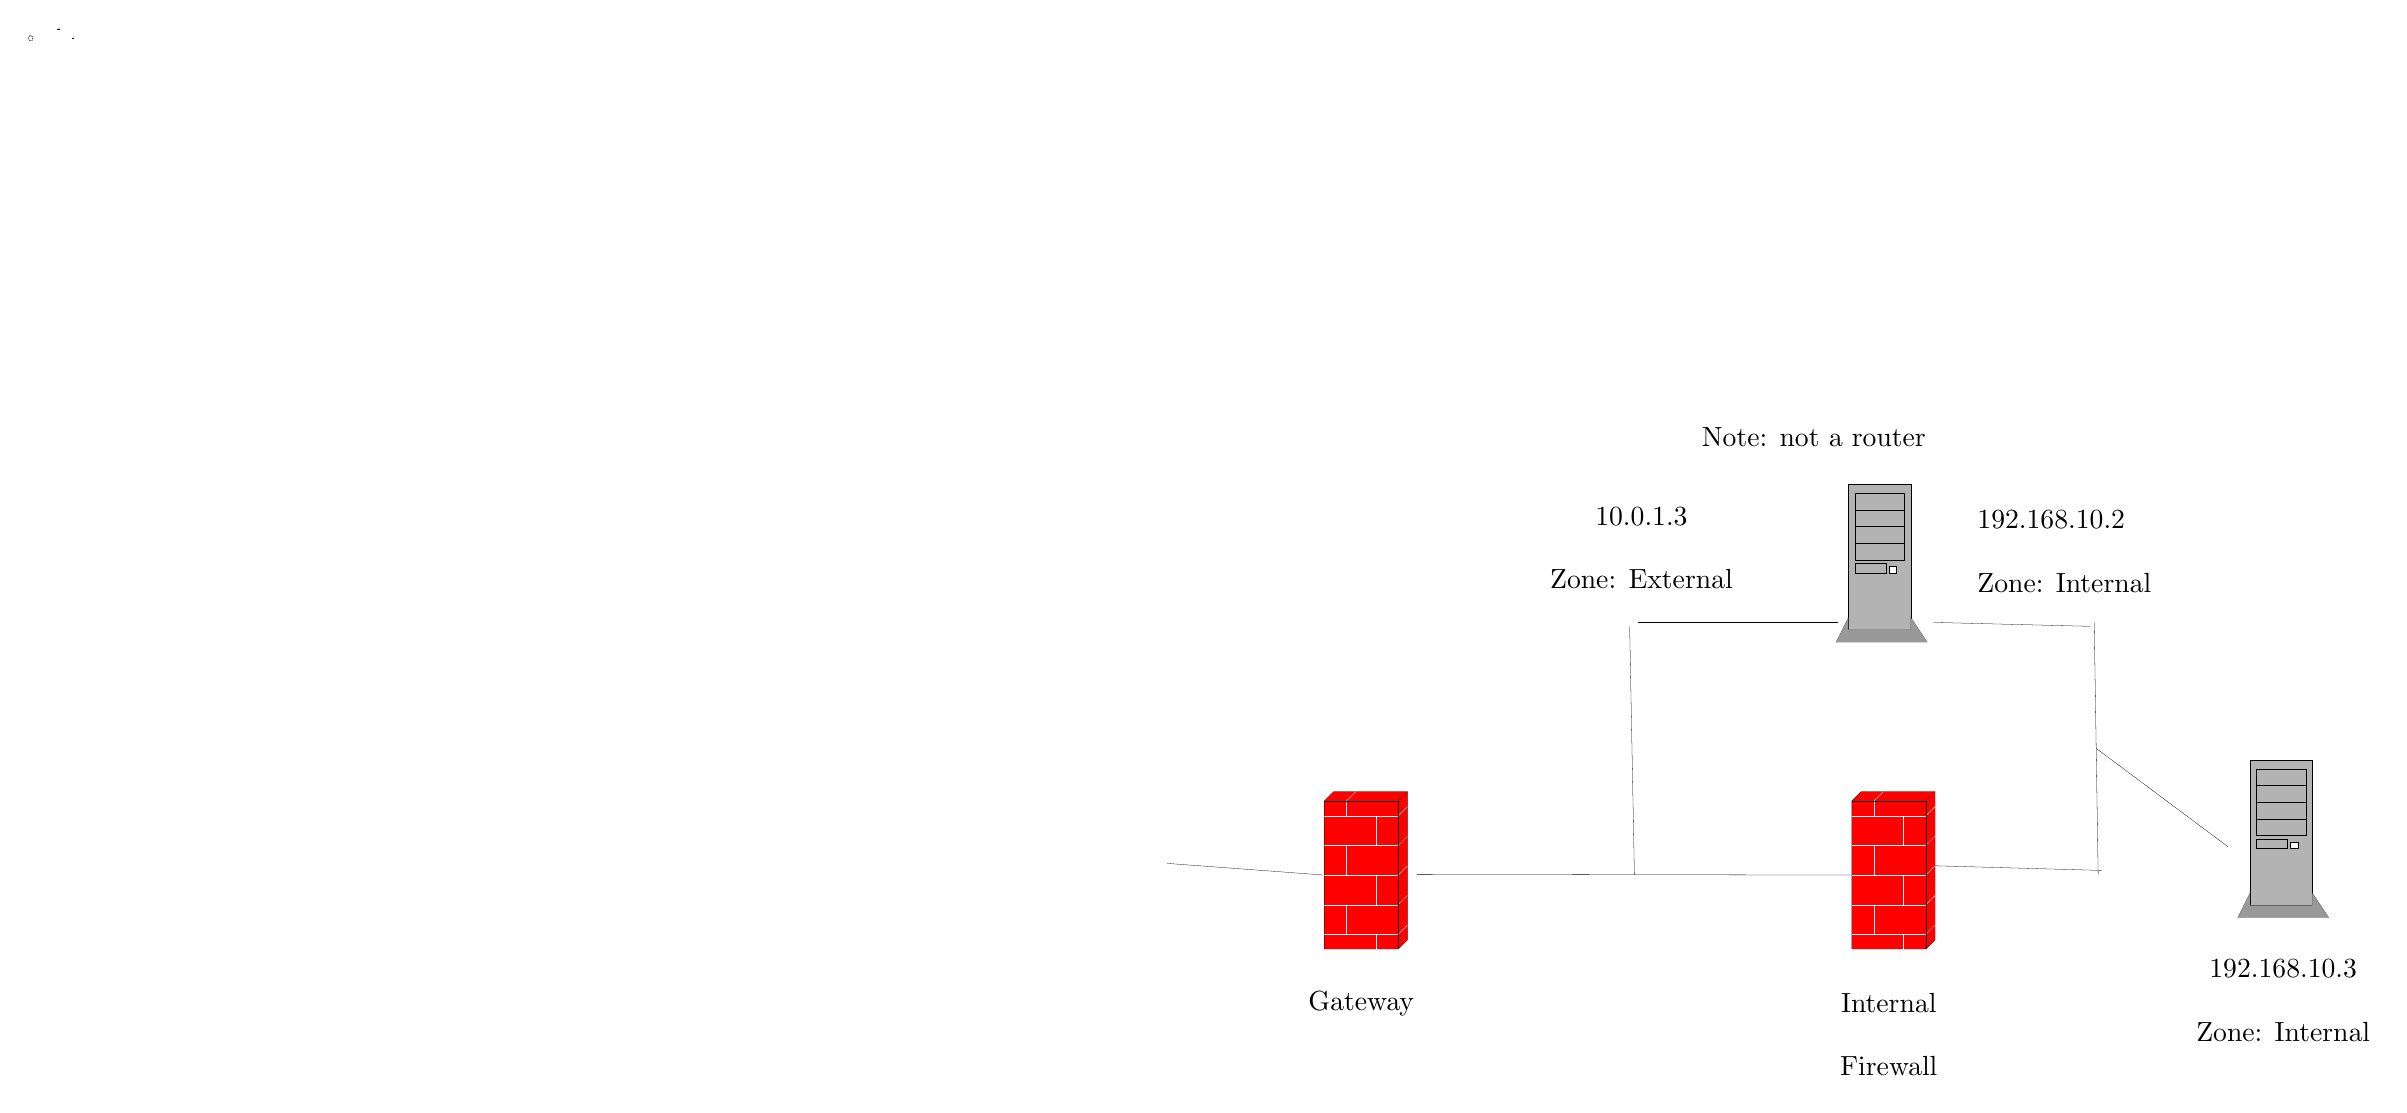
\begin{tikzpicture}
\pgftransformxscale{1.000000}
\pgftransformyscale{-1.000000}
\definecolor{dialinecolor}{rgb}{0.000000, 0.000000, 0.000000}
\pgfsetstrokecolor{dialinecolor}
\definecolor{dialinecolor}{rgb}{1.000000, 1.000000, 1.000000}
\pgfsetfillcolor{dialinecolor}
\pgfsetlinewidth{0.100000\du}
\pgfsetdash{}{0pt}
\pgfsetdash{}{0pt}
\pgfsetbuttcap
\pgfsetmiterjoin
\pgfsetlinewidth{0.100000\du}
\pgfsetbuttcap
\pgfsetmiterjoin
\pgfsetdash{}{0pt}
\definecolor{dialinecolor}{rgb}{1.000000, 0.000000, 0.000000}
\pgfsetfillcolor{dialinecolor}
\fill (16.920588\du,10.067647\du)--(16.920588\du,11.950000\du)--(17.861765\du,11.950000\du)--(17.861765\du,10.067647\du)--cycle;
\pgfsetbuttcap
\pgfsetmiterjoin
\pgfsetdash{}{0pt}
\definecolor{dialinecolor}{rgb}{1.000000, 0.000000, 0.000000}
\pgfsetfillcolor{dialinecolor}
\fill (16.920588\du,10.067647\du)--(17.861765\du,10.067647\du)--(17.979412\du,9.950000\du)--(17.038235\du,9.950000\du)--cycle;
\pgfsetbuttcap
\pgfsetmiterjoin
\pgfsetdash{}{0pt}
\definecolor{dialinecolor}{rgb}{1.000000, 0.000000, 0.000000}
\pgfsetfillcolor{dialinecolor}
\fill (17.861765\du,10.067647\du)--(17.979412\du,9.950000\du)--(17.979412\du,11.832353\du)--(17.861765\du,11.950000\du)--cycle;
\pgfsetbuttcap
\pgfsetmiterjoin
\pgfsetdash{}{0pt}
\definecolor{dialinecolor}{rgb}{1.000000, 1.000000, 1.000000}
\pgfsetstrokecolor{dialinecolor}
\draw (16.920588\du,10.255882\du)--(17.861765\du,10.255882\du);
\pgfsetbuttcap
\pgfsetmiterjoin
\pgfsetdash{}{0pt}
\definecolor{dialinecolor}{rgb}{1.000000, 1.000000, 1.000000}
\pgfsetstrokecolor{dialinecolor}
\draw (17.979412\du,10.138235\du)--(17.861765\du,10.255882\du);
\pgfsetbuttcap
\pgfsetmiterjoin
\pgfsetdash{}{0pt}
\definecolor{dialinecolor}{rgb}{1.000000, 1.000000, 1.000000}
\pgfsetstrokecolor{dialinecolor}
\draw (17.202941\du,10.067647\du)--(17.202941\du,10.255882\du);
\pgfsetbuttcap
\pgfsetmiterjoin
\pgfsetdash{}{0pt}
\definecolor{dialinecolor}{rgb}{1.000000, 1.000000, 1.000000}
\pgfsetstrokecolor{dialinecolor}
\draw (17.202941\du,10.067647\du)--(17.320588\du,9.950000\du);
\pgfsetbuttcap
\pgfsetmiterjoin
\pgfsetdash{}{0pt}
\definecolor{dialinecolor}{rgb}{1.000000, 1.000000, 1.000000}
\pgfsetstrokecolor{dialinecolor}
\draw (16.920588\du,10.632353\du)--(17.861765\du,10.632353\du);
\pgfsetbuttcap
\pgfsetmiterjoin
\pgfsetdash{}{0pt}
\definecolor{dialinecolor}{rgb}{1.000000, 1.000000, 1.000000}
\pgfsetstrokecolor{dialinecolor}
\draw (17.979412\du,10.514706\du)--(17.861765\du,10.632353\du);
\pgfsetbuttcap
\pgfsetmiterjoin
\pgfsetdash{}{0pt}
\definecolor{dialinecolor}{rgb}{1.000000, 1.000000, 1.000000}
\pgfsetstrokecolor{dialinecolor}
\draw (17.579412\du,10.255882\du)--(17.579412\du,10.632353\du);
\pgfsetbuttcap
\pgfsetmiterjoin
\pgfsetdash{}{0pt}
\definecolor{dialinecolor}{rgb}{1.000000, 1.000000, 1.000000}
\pgfsetstrokecolor{dialinecolor}
\draw (16.920588\du,11.008824\du)--(17.861765\du,11.008824\du);
\pgfsetbuttcap
\pgfsetmiterjoin
\pgfsetdash{}{0pt}
\definecolor{dialinecolor}{rgb}{1.000000, 1.000000, 1.000000}
\pgfsetstrokecolor{dialinecolor}
\draw (17.979412\du,10.891176\du)--(17.861765\du,11.008824\du);
\pgfsetbuttcap
\pgfsetmiterjoin
\pgfsetdash{}{0pt}
\definecolor{dialinecolor}{rgb}{1.000000, 1.000000, 1.000000}
\pgfsetstrokecolor{dialinecolor}
\draw (17.202941\du,10.632353\du)--(17.202941\du,11.008824\du);
\pgfsetbuttcap
\pgfsetmiterjoin
\pgfsetdash{}{0pt}
\definecolor{dialinecolor}{rgb}{1.000000, 1.000000, 1.000000}
\pgfsetstrokecolor{dialinecolor}
\draw (16.920588\du,11.385294\du)--(17.861765\du,11.385294\du);
\pgfsetbuttcap
\pgfsetmiterjoin
\pgfsetdash{}{0pt}
\definecolor{dialinecolor}{rgb}{1.000000, 1.000000, 1.000000}
\pgfsetstrokecolor{dialinecolor}
\draw (17.979412\du,11.267647\du)--(17.861765\du,11.385294\du);
\pgfsetbuttcap
\pgfsetmiterjoin
\pgfsetdash{}{0pt}
\definecolor{dialinecolor}{rgb}{1.000000, 1.000000, 1.000000}
\pgfsetstrokecolor{dialinecolor}
\draw (17.579412\du,11.008824\du)--(17.579412\du,11.385294\du);
\pgfsetbuttcap
\pgfsetmiterjoin
\pgfsetdash{}{0pt}
\definecolor{dialinecolor}{rgb}{1.000000, 1.000000, 1.000000}
\pgfsetstrokecolor{dialinecolor}
\draw (16.920588\du,11.761765\du)--(17.861765\du,11.761765\du);
\pgfsetbuttcap
\pgfsetmiterjoin
\pgfsetdash{}{0pt}
\definecolor{dialinecolor}{rgb}{1.000000, 1.000000, 1.000000}
\pgfsetstrokecolor{dialinecolor}
\draw (17.979412\du,11.644118\du)--(17.861765\du,11.761765\du);
\pgfsetbuttcap
\pgfsetmiterjoin
\pgfsetdash{}{0pt}
\definecolor{dialinecolor}{rgb}{1.000000, 1.000000, 1.000000}
\pgfsetstrokecolor{dialinecolor}
\draw (17.202941\du,11.385294\du)--(17.202941\du,11.761765\du);
\pgfsetbuttcap
\pgfsetmiterjoin
\pgfsetdash{}{0pt}
\definecolor{dialinecolor}{rgb}{1.000000, 1.000000, 1.000000}
\pgfsetstrokecolor{dialinecolor}
\draw (17.579412\du,11.761765\du)--(17.579412\du,11.950000\du);
\pgfsetlinewidth{0.050000\du}
\pgfsetbuttcap
\pgfsetmiterjoin
\pgfsetdash{}{0pt}
\definecolor{dialinecolor}{rgb}{0.000000, 0.000000, 0.000000}
\pgfsetstrokecolor{dialinecolor}
\draw (16.920588\du,10.067647\du)--(17.861765\du,10.067647\du);
\pgfsetbuttcap
\pgfsetmiterjoin
\pgfsetdash{}{0pt}
\definecolor{dialinecolor}{rgb}{0.000000, 0.000000, 0.000000}
\pgfsetstrokecolor{dialinecolor}
\draw (17.861765\du,11.950000\du)--(17.861765\du,10.067647\du);
\pgfsetbuttcap
\pgfsetmiterjoin
\pgfsetdash{}{0pt}
\definecolor{dialinecolor}{rgb}{0.000000, 0.000000, 0.000000}
\pgfsetstrokecolor{dialinecolor}
\draw (17.861765\du,10.067647\du)--(17.979412\du,9.950000\du);
\pgfsetbuttcap
\pgfsetmiterjoin
\pgfsetdash{}{0pt}
\definecolor{dialinecolor}{rgb}{0.000000, 0.000000, 0.000000}
\pgfsetstrokecolor{dialinecolor}
\draw (16.920588\du,10.067647\du)--(17.038235\du,9.950000\du)--(17.979412\du,9.950000\du)--(17.979412\du,11.832353\du)--(17.861765\du,11.950000\du)--(16.920588\du,11.950000\du)--(16.920588\du,10.067647\du);
% setfont left to latex
\definecolor{dialinecolor}{rgb}{0.000000, 0.000000, 0.000000}
\pgfsetstrokecolor{dialinecolor}
\node at (17.391176\du,12.638161\du){Gateway};
\pgfsetlinewidth{0.100000\du}
\pgfsetdash{}{0pt}
\pgfsetdash{}{0pt}
\pgfsetbuttcap
\pgfsetmiterjoin
\pgfsetlinewidth{0.100000\du}
\pgfsetbuttcap
\pgfsetmiterjoin
\pgfsetdash{}{0pt}
\definecolor{dialinecolor}{rgb}{1.000000, 0.000000, 0.000000}
\pgfsetfillcolor{dialinecolor}
\fill (23.620588\du,10.067647\du)--(23.620588\du,11.950000\du)--(24.561765\du,11.950000\du)--(24.561765\du,10.067647\du)--cycle;
\pgfsetbuttcap
\pgfsetmiterjoin
\pgfsetdash{}{0pt}
\definecolor{dialinecolor}{rgb}{1.000000, 0.000000, 0.000000}
\pgfsetfillcolor{dialinecolor}
\fill (23.620588\du,10.067647\du)--(24.561765\du,10.067647\du)--(24.679412\du,9.950000\du)--(23.738235\du,9.950000\du)--cycle;
\pgfsetbuttcap
\pgfsetmiterjoin
\pgfsetdash{}{0pt}
\definecolor{dialinecolor}{rgb}{1.000000, 0.000000, 0.000000}
\pgfsetfillcolor{dialinecolor}
\fill (24.561765\du,10.067647\du)--(24.679412\du,9.950000\du)--(24.679412\du,11.832353\du)--(24.561765\du,11.950000\du)--cycle;
\pgfsetbuttcap
\pgfsetmiterjoin
\pgfsetdash{}{0pt}
\definecolor{dialinecolor}{rgb}{1.000000, 1.000000, 1.000000}
\pgfsetstrokecolor{dialinecolor}
\draw (23.620588\du,10.255882\du)--(24.561765\du,10.255882\du);
\pgfsetbuttcap
\pgfsetmiterjoin
\pgfsetdash{}{0pt}
\definecolor{dialinecolor}{rgb}{1.000000, 1.000000, 1.000000}
\pgfsetstrokecolor{dialinecolor}
\draw (24.679412\du,10.138235\du)--(24.561765\du,10.255882\du);
\pgfsetbuttcap
\pgfsetmiterjoin
\pgfsetdash{}{0pt}
\definecolor{dialinecolor}{rgb}{1.000000, 1.000000, 1.000000}
\pgfsetstrokecolor{dialinecolor}
\draw (23.902941\du,10.067647\du)--(23.902941\du,10.255882\du);
\pgfsetbuttcap
\pgfsetmiterjoin
\pgfsetdash{}{0pt}
\definecolor{dialinecolor}{rgb}{1.000000, 1.000000, 1.000000}
\pgfsetstrokecolor{dialinecolor}
\draw (23.902941\du,10.067647\du)--(24.020588\du,9.950000\du);
\pgfsetbuttcap
\pgfsetmiterjoin
\pgfsetdash{}{0pt}
\definecolor{dialinecolor}{rgb}{1.000000, 1.000000, 1.000000}
\pgfsetstrokecolor{dialinecolor}
\draw (23.620588\du,10.632353\du)--(24.561765\du,10.632353\du);
\pgfsetbuttcap
\pgfsetmiterjoin
\pgfsetdash{}{0pt}
\definecolor{dialinecolor}{rgb}{1.000000, 1.000000, 1.000000}
\pgfsetstrokecolor{dialinecolor}
\draw (24.679412\du,10.514706\du)--(24.561765\du,10.632353\du);
\pgfsetbuttcap
\pgfsetmiterjoin
\pgfsetdash{}{0pt}
\definecolor{dialinecolor}{rgb}{1.000000, 1.000000, 1.000000}
\pgfsetstrokecolor{dialinecolor}
\draw (24.279412\du,10.255882\du)--(24.279412\du,10.632353\du);
\pgfsetbuttcap
\pgfsetmiterjoin
\pgfsetdash{}{0pt}
\definecolor{dialinecolor}{rgb}{1.000000, 1.000000, 1.000000}
\pgfsetstrokecolor{dialinecolor}
\draw (23.620588\du,11.008824\du)--(24.561765\du,11.008824\du);
\pgfsetbuttcap
\pgfsetmiterjoin
\pgfsetdash{}{0pt}
\definecolor{dialinecolor}{rgb}{1.000000, 1.000000, 1.000000}
\pgfsetstrokecolor{dialinecolor}
\draw (24.679412\du,10.891176\du)--(24.561765\du,11.008824\du);
\pgfsetbuttcap
\pgfsetmiterjoin
\pgfsetdash{}{0pt}
\definecolor{dialinecolor}{rgb}{1.000000, 1.000000, 1.000000}
\pgfsetstrokecolor{dialinecolor}
\draw (23.902941\du,10.632353\du)--(23.902941\du,11.008824\du);
\pgfsetbuttcap
\pgfsetmiterjoin
\pgfsetdash{}{0pt}
\definecolor{dialinecolor}{rgb}{1.000000, 1.000000, 1.000000}
\pgfsetstrokecolor{dialinecolor}
\draw (23.620588\du,11.385294\du)--(24.561765\du,11.385294\du);
\pgfsetbuttcap
\pgfsetmiterjoin
\pgfsetdash{}{0pt}
\definecolor{dialinecolor}{rgb}{1.000000, 1.000000, 1.000000}
\pgfsetstrokecolor{dialinecolor}
\draw (24.679412\du,11.267647\du)--(24.561765\du,11.385294\du);
\pgfsetbuttcap
\pgfsetmiterjoin
\pgfsetdash{}{0pt}
\definecolor{dialinecolor}{rgb}{1.000000, 1.000000, 1.000000}
\pgfsetstrokecolor{dialinecolor}
\draw (24.279412\du,11.008824\du)--(24.279412\du,11.385294\du);
\pgfsetbuttcap
\pgfsetmiterjoin
\pgfsetdash{}{0pt}
\definecolor{dialinecolor}{rgb}{1.000000, 1.000000, 1.000000}
\pgfsetstrokecolor{dialinecolor}
\draw (23.620588\du,11.761765\du)--(24.561765\du,11.761765\du);
\pgfsetbuttcap
\pgfsetmiterjoin
\pgfsetdash{}{0pt}
\definecolor{dialinecolor}{rgb}{1.000000, 1.000000, 1.000000}
\pgfsetstrokecolor{dialinecolor}
\draw (24.679412\du,11.644118\du)--(24.561765\du,11.761765\du);
\pgfsetbuttcap
\pgfsetmiterjoin
\pgfsetdash{}{0pt}
\definecolor{dialinecolor}{rgb}{1.000000, 1.000000, 1.000000}
\pgfsetstrokecolor{dialinecolor}
\draw (23.902941\du,11.385294\du)--(23.902941\du,11.761765\du);
\pgfsetbuttcap
\pgfsetmiterjoin
\pgfsetdash{}{0pt}
\definecolor{dialinecolor}{rgb}{1.000000, 1.000000, 1.000000}
\pgfsetstrokecolor{dialinecolor}
\draw (24.279412\du,11.761765\du)--(24.279412\du,11.950000\du);
\pgfsetlinewidth{0.050000\du}
\pgfsetbuttcap
\pgfsetmiterjoin
\pgfsetdash{}{0pt}
\definecolor{dialinecolor}{rgb}{0.000000, 0.000000, 0.000000}
\pgfsetstrokecolor{dialinecolor}
\draw (23.620588\du,10.067647\du)--(24.561765\du,10.067647\du);
\pgfsetbuttcap
\pgfsetmiterjoin
\pgfsetdash{}{0pt}
\definecolor{dialinecolor}{rgb}{0.000000, 0.000000, 0.000000}
\pgfsetstrokecolor{dialinecolor}
\draw (24.561765\du,11.950000\du)--(24.561765\du,10.067647\du);
\pgfsetbuttcap
\pgfsetmiterjoin
\pgfsetdash{}{0pt}
\definecolor{dialinecolor}{rgb}{0.000000, 0.000000, 0.000000}
\pgfsetstrokecolor{dialinecolor}
\draw (24.561765\du,10.067647\du)--(24.679412\du,9.950000\du);
\pgfsetbuttcap
\pgfsetmiterjoin
\pgfsetdash{}{0pt}
\definecolor{dialinecolor}{rgb}{0.000000, 0.000000, 0.000000}
\pgfsetstrokecolor{dialinecolor}
\draw (23.620588\du,10.067647\du)--(23.738235\du,9.950000\du)--(24.679412\du,9.950000\du)--(24.679412\du,11.832353\du)--(24.561765\du,11.950000\du)--(23.620588\du,11.950000\du)--(23.620588\du,10.067647\du);
% setfont left to latex
\definecolor{dialinecolor}{rgb}{0.000000, 0.000000, 0.000000}
\pgfsetstrokecolor{dialinecolor}
\node at (24.091176\du,12.638161\du){Internal};
% setfont left to latex
\definecolor{dialinecolor}{rgb}{0.000000, 0.000000, 0.000000}
\pgfsetstrokecolor{dialinecolor}
\node at (24.091176\du,13.438161\du){Firewall};
\pgfsetlinewidth{0.100000\du}
\pgfsetdash{}{0pt}
\pgfsetdash{}{0pt}
\pgfsetbuttcap
\pgfsetmiterjoin
\pgfsetlinewidth{0.080000\du}
\pgfsetbuttcap
\pgfsetmiterjoin
\pgfsetdash{}{0pt}
\definecolor{dialinecolor}{rgb}{0.701961, 0.701961, 0.701961}
\pgfsetfillcolor{dialinecolor}
\fill (23.578947\du,6.050000\du)--(23.578947\du,7.892105\du)--(24.368421\du,7.892105\du)--(24.368421\du,6.050000\du)--cycle;
\definecolor{dialinecolor}{rgb}{0.000000, 0.000000, 0.000000}
\pgfsetstrokecolor{dialinecolor}
\draw (23.578947\du,6.050000\du)--(23.578947\du,7.892105\du)--(24.368421\du,7.892105\du)--(24.368421\du,6.050000\du)--cycle;
\pgfsetlinewidth{0.010000\du}
\pgfsetbuttcap
\pgfsetmiterjoin
\pgfsetdash{}{0pt}
\definecolor{dialinecolor}{rgb}{0.000000, 0.000000, 0.000000}
\pgfsetstrokecolor{dialinecolor}
\draw (23.657895\du,6.160526\du)--(23.657895\du,6.371053\du)--(24.289474\du,6.371053\du)--(24.289474\du,6.160526\du)--cycle;
\pgfsetbuttcap
\pgfsetmiterjoin
\pgfsetdash{}{0pt}
\definecolor{dialinecolor}{rgb}{0.000000, 0.000000, 0.000000}
\pgfsetstrokecolor{dialinecolor}
\draw (23.657895\du,6.371053\du)--(23.657895\du,6.581579\du)--(24.289474\du,6.581579\du)--(24.289474\du,6.371053\du)--cycle;
\pgfsetbuttcap
\pgfsetmiterjoin
\pgfsetdash{}{0pt}
\definecolor{dialinecolor}{rgb}{0.000000, 0.000000, 0.000000}
\pgfsetstrokecolor{dialinecolor}
\draw (23.657895\du,6.581579\du)--(23.657895\du,6.792105\du)--(24.289474\du,6.792105\du)--(24.289474\du,6.581579\du)--cycle;
\pgfsetbuttcap
\pgfsetmiterjoin
\pgfsetdash{}{0pt}
\definecolor{dialinecolor}{rgb}{0.000000, 0.000000, 0.000000}
\pgfsetstrokecolor{dialinecolor}
\draw (23.657895\du,6.792105\du)--(23.657895\du,7.002632\du)--(24.289474\du,7.002632\du)--(24.289474\du,6.792105\du)--cycle;
\pgfsetbuttcap
\pgfsetmiterjoin
\pgfsetdash{}{0pt}
\definecolor{dialinecolor}{rgb}{0.000000, 0.000000, 0.000000}
\pgfsetstrokecolor{dialinecolor}
\draw (23.657895\du,7.044737\du)--(23.657895\du,7.171053\du)--(24.052632\du,7.171053\du)--(24.052632\du,7.044737\du)--cycle;
\pgfsetbuttcap
\pgfsetmiterjoin
\pgfsetdash{}{0pt}
\definecolor{dialinecolor}{rgb}{0.000000, 1.000000, 0.000000}
\pgfsetfillcolor{dialinecolor}
\pgfpathellipse{\pgfpoint{24.250000\du}{7.065789\du}}{\pgfpoint{0.027632\du}{0\du}}{\pgfpoint{0\du}{0.027632\du}}
\pgfusepath{fill}
\definecolor{dialinecolor}{rgb}{0.000000, 0.000000, 0.000000}
\pgfsetstrokecolor{dialinecolor}
\pgfpathellipse{\pgfpoint{24.250000\du}{7.065789\du}}{\pgfpoint{0.027632\du}{0\du}}{\pgfpoint{0\du}{0.027632\du}}
\pgfusepath{stroke}
\pgfsetbuttcap
\pgfsetmiterjoin
\pgfsetdash{}{0pt}
\definecolor{dialinecolor}{rgb}{1.000000, 1.000000, 0.000000}
\pgfsetfillcolor{dialinecolor}
\pgfpathellipse{\pgfpoint{24.250000\du}{7.150000\du}}{\pgfpoint{0.027632\du}{0\du}}{\pgfpoint{0\du}{0.027632\du}}
\pgfusepath{fill}
\definecolor{dialinecolor}{rgb}{0.000000, 0.000000, 0.000000}
\pgfsetstrokecolor{dialinecolor}
\pgfpathellipse{\pgfpoint{24.250000\du}{7.150000\du}}{\pgfpoint{0.027632\du}{0\du}}{\pgfpoint{0\du}{0.027632\du}}
\pgfusepath{stroke}
\pgfsetbuttcap
\pgfsetmiterjoin
\pgfsetdash{}{0pt}
\definecolor{dialinecolor}{rgb}{1.000000, 1.000000, 1.000000}
\pgfsetfillcolor{dialinecolor}
\fill (24.092105\du,7.086842\du)--(24.092105\du,7.171053\du)--(24.186842\du,7.171053\du)--(24.186842\du,7.086842\du)--cycle;
\definecolor{dialinecolor}{rgb}{0.000000, 0.000000, 0.000000}
\pgfsetstrokecolor{dialinecolor}
\draw (24.092105\du,7.086842\du)--(24.092105\du,7.171053\du)--(24.186842\du,7.171053\du)--(24.186842\du,7.086842\du)--cycle;
\pgfsetbuttcap
\pgfsetmiterjoin
\pgfsetdash{}{0pt}
\definecolor{dialinecolor}{rgb}{0.000000, 0.000000, 0.000000}
\pgfsetstrokecolor{dialinecolor}
\pgfpathmoveto{\pgfpoint{23.710526\du}{7.339474\du}}
\pgfpathlineto{\pgfpoint{23.710526\du}{7.800000\du}}
\pgfusepath{stroke}
\pgfsetbuttcap
\pgfsetmiterjoin
\pgfsetdash{}{0pt}
\definecolor{dialinecolor}{rgb}{0.000000, 0.000000, 0.000000}
\pgfsetstrokecolor{dialinecolor}
\pgfpathmoveto{\pgfpoint{23.842105\du}{7.339474\du}}
\pgfpathlineto{\pgfpoint{23.842105\du}{7.800000\du}}
\pgfusepath{stroke}
\pgfsetbuttcap
\pgfsetmiterjoin
\pgfsetdash{}{0pt}
\definecolor{dialinecolor}{rgb}{0.000000, 0.000000, 0.000000}
\pgfsetstrokecolor{dialinecolor}
\pgfpathmoveto{\pgfpoint{23.973684\du}{7.339474\du}}
\pgfpathlineto{\pgfpoint{23.973684\du}{7.800000\du}}
\pgfusepath{stroke}
\pgfsetbuttcap
\pgfsetmiterjoin
\pgfsetdash{}{0pt}
\definecolor{dialinecolor}{rgb}{0.000000, 0.000000, 0.000000}
\pgfsetstrokecolor{dialinecolor}
\pgfpathmoveto{\pgfpoint{24.105263\du}{7.339474\du}}
\pgfpathlineto{\pgfpoint{24.105263\du}{7.800000\du}}
\pgfusepath{stroke}
\pgfsetbuttcap
\pgfsetmiterjoin
\pgfsetdash{}{0pt}
\definecolor{dialinecolor}{rgb}{0.000000, 0.000000, 0.000000}
\pgfsetstrokecolor{dialinecolor}
\pgfpathmoveto{\pgfpoint{24.236842\du}{7.339474\du}}
\pgfpathlineto{\pgfpoint{24.236842\du}{7.800000\du}}
\pgfusepath{stroke}
\pgfsetbuttcap
\pgfsetmiterjoin
\pgfsetdash{}{0pt}
\definecolor{dialinecolor}{rgb}{0.000000, 0.000000, 0.000000}
\pgfsetstrokecolor{dialinecolor}
\pgfpathmoveto{\pgfpoint{24.368421\du}{7.339474\du}}
\pgfpathlineto{\pgfpoint{24.368421\du}{7.800000\du}}
\pgfusepath{stroke}
\pgfsetbuttcap
\pgfsetmiterjoin
\pgfsetdash{}{0pt}
\definecolor{dialinecolor}{rgb}{0.600000, 0.600000, 0.600000}
\pgfsetfillcolor{dialinecolor}
\fill (23.421053\du,8.050000\du)--(23.578947\du,7.734211\du)--(23.578947\du,7.892105\du)--(24.368421\du,7.892105\du)--(24.368421\du,7.734211\du)--(24.578947\du,8.050000\du)--cycle;
\definecolor{dialinecolor}{rgb}{0.000000, 0.000000, 0.000000}
\pgfsetstrokecolor{dialinecolor}
\draw (23.421053\du,8.050000\du)--(23.578947\du,7.734211\du)--(23.578947\du,7.892105\du)--(24.368421\du,7.892105\du)--(24.368421\du,7.734211\du)--(24.578947\du,8.050000\du)--cycle;
% setfont left to latex
\definecolor{dialinecolor}{rgb}{0.000000, 0.000000, 0.000000}
\pgfsetstrokecolor{dialinecolor}
\node at (24.000000\du,8.696675\du){};
\pgfsetlinewidth{0.100000\du}
\pgfsetdash{}{0pt}
\pgfsetdash{}{0pt}
\pgfsetbuttcap
{
\definecolor{dialinecolor}{rgb}{0.000000, 0.000000, 0.000000}
\pgfsetfillcolor{dialinecolor}
% was here!!!
\definecolor{dialinecolor}{rgb}{0.000000, 0.000000, 0.000000}
\pgfsetstrokecolor{dialinecolor}
\draw (18.100000\du,11.000000\du)--(23.620588\du,11.008824\du);
}
\pgfsetlinewidth{0.100000\du}
\pgfsetdash{}{0pt}
\pgfsetdash{}{0pt}
\pgfsetbuttcap
{
\definecolor{dialinecolor}{rgb}{0.000000, 0.000000, 0.000000}
\pgfsetfillcolor{dialinecolor}
% was here!!!
\definecolor{dialinecolor}{rgb}{0.000000, 0.000000, 0.000000}
\pgfsetstrokecolor{dialinecolor}
\draw (20.860294\du,11.004412\du)--(20.800000\du,7.850000\du);
}
\pgfsetlinewidth{0.100000\du}
\pgfsetdash{}{0pt}
\pgfsetdash{}{0pt}
\pgfsetbuttcap
{
\definecolor{dialinecolor}{rgb}{0.000000, 0.000000, 0.000000}
\pgfsetfillcolor{dialinecolor}
% was here!!!
\definecolor{dialinecolor}{rgb}{0.000000, 0.000000, 0.000000}
\pgfsetstrokecolor{dialinecolor}
\draw (20.900000\du,7.800000\du)--(23.450000\du,7.800000\du);
}
\pgfsetlinewidth{0.100000\du}
\pgfsetdash{}{0pt}
\pgfsetdash{}{0pt}
\pgfsetbuttcap
{
\definecolor{dialinecolor}{rgb}{0.000000, 0.000000, 0.000000}
\pgfsetfillcolor{dialinecolor}
% was here!!!
\definecolor{dialinecolor}{rgb}{0.000000, 0.000000, 0.000000}
\pgfsetstrokecolor{dialinecolor}
\draw (24.679412\du,10.891176\du)--(26.800000\du,10.950000\du);
}
\pgfsetlinewidth{0.100000\du}
\pgfsetdash{}{0pt}
\pgfsetdash{}{0pt}
\pgfsetbuttcap
{
\definecolor{dialinecolor}{rgb}{0.000000, 0.000000, 0.000000}
\pgfsetfillcolor{dialinecolor}
% was here!!!
\definecolor{dialinecolor}{rgb}{0.000000, 0.000000, 0.000000}
\pgfsetstrokecolor{dialinecolor}
\draw (26.750000\du,11.000000\du)--(26.700000\du,7.800000\du);
}
\pgfsetlinewidth{0.100000\du}
\pgfsetdash{}{0pt}
\pgfsetdash{}{0pt}
\pgfsetbuttcap
{
\definecolor{dialinecolor}{rgb}{0.000000, 0.000000, 0.000000}
\pgfsetfillcolor{dialinecolor}
% was here!!!
\definecolor{dialinecolor}{rgb}{0.000000, 0.000000, 0.000000}
\pgfsetstrokecolor{dialinecolor}
\draw (26.650000\du,7.850000\du)--(24.650000\du,7.800000\du);
}
\pgfsetlinewidth{0.100000\du}
\pgfsetdash{}{0pt}
\pgfsetdash{}{0pt}
\pgfsetbuttcap
\pgfsetmiterjoin
\pgfsetlinewidth{0.080000\du}
\pgfsetbuttcap
\pgfsetmiterjoin
\pgfsetdash{}{0pt}
\definecolor{dialinecolor}{rgb}{0.701961, 0.701961, 0.701961}
\pgfsetfillcolor{dialinecolor}
\fill (28.678947\du,9.550000\du)--(28.678947\du,11.392105\du)--(29.468421\du,11.392105\du)--(29.468421\du,9.550000\du)--cycle;
\definecolor{dialinecolor}{rgb}{0.000000, 0.000000, 0.000000}
\pgfsetstrokecolor{dialinecolor}
\draw (28.678947\du,9.550000\du)--(28.678947\du,11.392105\du)--(29.468421\du,11.392105\du)--(29.468421\du,9.550000\du)--cycle;
\pgfsetlinewidth{0.010000\du}
\pgfsetbuttcap
\pgfsetmiterjoin
\pgfsetdash{}{0pt}
\definecolor{dialinecolor}{rgb}{0.000000, 0.000000, 0.000000}
\pgfsetstrokecolor{dialinecolor}
\draw (28.757895\du,9.660526\du)--(28.757895\du,9.871053\du)--(29.389474\du,9.871053\du)--(29.389474\du,9.660526\du)--cycle;
\pgfsetbuttcap
\pgfsetmiterjoin
\pgfsetdash{}{0pt}
\definecolor{dialinecolor}{rgb}{0.000000, 0.000000, 0.000000}
\pgfsetstrokecolor{dialinecolor}
\draw (28.757895\du,9.871053\du)--(28.757895\du,10.081579\du)--(29.389474\du,10.081579\du)--(29.389474\du,9.871053\du)--cycle;
\pgfsetbuttcap
\pgfsetmiterjoin
\pgfsetdash{}{0pt}
\definecolor{dialinecolor}{rgb}{0.000000, 0.000000, 0.000000}
\pgfsetstrokecolor{dialinecolor}
\draw (28.757895\du,10.081579\du)--(28.757895\du,10.292105\du)--(29.389474\du,10.292105\du)--(29.389474\du,10.081579\du)--cycle;
\pgfsetbuttcap
\pgfsetmiterjoin
\pgfsetdash{}{0pt}
\definecolor{dialinecolor}{rgb}{0.000000, 0.000000, 0.000000}
\pgfsetstrokecolor{dialinecolor}
\draw (28.757895\du,10.292105\du)--(28.757895\du,10.502632\du)--(29.389474\du,10.502632\du)--(29.389474\du,10.292105\du)--cycle;
\pgfsetbuttcap
\pgfsetmiterjoin
\pgfsetdash{}{0pt}
\definecolor{dialinecolor}{rgb}{0.000000, 0.000000, 0.000000}
\pgfsetstrokecolor{dialinecolor}
\draw (28.757895\du,10.544737\du)--(28.757895\du,10.671053\du)--(29.152632\du,10.671053\du)--(29.152632\du,10.544737\du)--cycle;
\pgfsetbuttcap
\pgfsetmiterjoin
\pgfsetdash{}{0pt}
\definecolor{dialinecolor}{rgb}{0.000000, 1.000000, 0.000000}
\pgfsetfillcolor{dialinecolor}
\pgfpathellipse{\pgfpoint{29.350000\du}{10.565789\du}}{\pgfpoint{0.027632\du}{0\du}}{\pgfpoint{0\du}{0.027632\du}}
\pgfusepath{fill}
\definecolor{dialinecolor}{rgb}{0.000000, 0.000000, 0.000000}
\pgfsetstrokecolor{dialinecolor}
\pgfpathellipse{\pgfpoint{29.350000\du}{10.565789\du}}{\pgfpoint{0.027632\du}{0\du}}{\pgfpoint{0\du}{0.027632\du}}
\pgfusepath{stroke}
\pgfsetbuttcap
\pgfsetmiterjoin
\pgfsetdash{}{0pt}
\definecolor{dialinecolor}{rgb}{1.000000, 1.000000, 0.000000}
\pgfsetfillcolor{dialinecolor}
\pgfpathellipse{\pgfpoint{29.350000\du}{10.650000\du}}{\pgfpoint{0.027632\du}{0\du}}{\pgfpoint{0\du}{0.027632\du}}
\pgfusepath{fill}
\definecolor{dialinecolor}{rgb}{0.000000, 0.000000, 0.000000}
\pgfsetstrokecolor{dialinecolor}
\pgfpathellipse{\pgfpoint{29.350000\du}{10.650000\du}}{\pgfpoint{0.027632\du}{0\du}}{\pgfpoint{0\du}{0.027632\du}}
\pgfusepath{stroke}
\pgfsetbuttcap
\pgfsetmiterjoin
\pgfsetdash{}{0pt}
\definecolor{dialinecolor}{rgb}{1.000000, 1.000000, 1.000000}
\pgfsetfillcolor{dialinecolor}
\fill (29.192105\du,10.586842\du)--(29.192105\du,10.671053\du)--(29.286842\du,10.671053\du)--(29.286842\du,10.586842\du)--cycle;
\definecolor{dialinecolor}{rgb}{0.000000, 0.000000, 0.000000}
\pgfsetstrokecolor{dialinecolor}
\draw (29.192105\du,10.586842\du)--(29.192105\du,10.671053\du)--(29.286842\du,10.671053\du)--(29.286842\du,10.586842\du)--cycle;
\pgfsetbuttcap
\pgfsetmiterjoin
\pgfsetdash{}{0pt}
\definecolor{dialinecolor}{rgb}{0.000000, 0.000000, 0.000000}
\pgfsetstrokecolor{dialinecolor}
\pgfpathmoveto{\pgfpoint{28.810526\du}{10.839474\du}}
\pgfpathlineto{\pgfpoint{28.810526\du}{11.300000\du}}
\pgfusepath{stroke}
\pgfsetbuttcap
\pgfsetmiterjoin
\pgfsetdash{}{0pt}
\definecolor{dialinecolor}{rgb}{0.000000, 0.000000, 0.000000}
\pgfsetstrokecolor{dialinecolor}
\pgfpathmoveto{\pgfpoint{28.942105\du}{10.839474\du}}
\pgfpathlineto{\pgfpoint{28.942105\du}{11.300000\du}}
\pgfusepath{stroke}
\pgfsetbuttcap
\pgfsetmiterjoin
\pgfsetdash{}{0pt}
\definecolor{dialinecolor}{rgb}{0.000000, 0.000000, 0.000000}
\pgfsetstrokecolor{dialinecolor}
\pgfpathmoveto{\pgfpoint{29.073684\du}{10.839474\du}}
\pgfpathlineto{\pgfpoint{29.073684\du}{11.300000\du}}
\pgfusepath{stroke}
\pgfsetbuttcap
\pgfsetmiterjoin
\pgfsetdash{}{0pt}
\definecolor{dialinecolor}{rgb}{0.000000, 0.000000, 0.000000}
\pgfsetstrokecolor{dialinecolor}
\pgfpathmoveto{\pgfpoint{29.205263\du}{10.839474\du}}
\pgfpathlineto{\pgfpoint{29.205263\du}{11.300000\du}}
\pgfusepath{stroke}
\pgfsetbuttcap
\pgfsetmiterjoin
\pgfsetdash{}{0pt}
\definecolor{dialinecolor}{rgb}{0.000000, 0.000000, 0.000000}
\pgfsetstrokecolor{dialinecolor}
\pgfpathmoveto{\pgfpoint{29.336842\du}{10.839474\du}}
\pgfpathlineto{\pgfpoint{29.336842\du}{11.300000\du}}
\pgfusepath{stroke}
\pgfsetbuttcap
\pgfsetmiterjoin
\pgfsetdash{}{0pt}
\definecolor{dialinecolor}{rgb}{0.000000, 0.000000, 0.000000}
\pgfsetstrokecolor{dialinecolor}
\pgfpathmoveto{\pgfpoint{29.468421\du}{10.839474\du}}
\pgfpathlineto{\pgfpoint{29.468421\du}{11.300000\du}}
\pgfusepath{stroke}
\pgfsetbuttcap
\pgfsetmiterjoin
\pgfsetdash{}{0pt}
\definecolor{dialinecolor}{rgb}{0.600000, 0.600000, 0.600000}
\pgfsetfillcolor{dialinecolor}
\fill (28.521053\du,11.550000\du)--(28.678947\du,11.234211\du)--(28.678947\du,11.392105\du)--(29.468421\du,11.392105\du)--(29.468421\du,11.234211\du)--(29.678947\du,11.550000\du)--cycle;
\definecolor{dialinecolor}{rgb}{0.000000, 0.000000, 0.000000}
\pgfsetstrokecolor{dialinecolor}
\draw (28.521053\du,11.550000\du)--(28.678947\du,11.234211\du)--(28.678947\du,11.392105\du)--(29.468421\du,11.392105\du)--(29.468421\du,11.234211\du)--(29.678947\du,11.550000\du)--cycle;
% setfont left to latex
\definecolor{dialinecolor}{rgb}{0.000000, 0.000000, 0.000000}
\pgfsetstrokecolor{dialinecolor}
\node at (29.100000\du,12.196675\du){192.168.10.3};
% setfont left to latex
\definecolor{dialinecolor}{rgb}{0.000000, 0.000000, 0.000000}
\pgfsetstrokecolor{dialinecolor}
\node at (29.100000\du,12.996675\du){Zone: Internal};
% setfont left to latex
\definecolor{dialinecolor}{rgb}{0.000000, 0.000000, 0.000000}
\pgfsetstrokecolor{dialinecolor}
\node[anchor=west] at (25.100000\du,6.500000\du){192.168.10.2};
% setfont left to latex
\definecolor{dialinecolor}{rgb}{0.000000, 0.000000, 0.000000}
\pgfsetstrokecolor{dialinecolor}
\node[anchor=west] at (25.100000\du,7.300000\du){Zone: Internal};
% setfont left to latex
\definecolor{dialinecolor}{rgb}{0.000000, 0.000000, 0.000000}
\pgfsetstrokecolor{dialinecolor}
\node at (20.950000\du,6.450000\du){10.0.1.3};
% setfont left to latex
\definecolor{dialinecolor}{rgb}{0.000000, 0.000000, 0.000000}
\pgfsetstrokecolor{dialinecolor}
\node at (20.950000\du,7.250000\du){Zone: External};
\pgfsetlinewidth{0.100000\du}
\pgfsetdash{}{0pt}
\pgfsetdash{}{0pt}
\pgfsetbuttcap
{
\definecolor{dialinecolor}{rgb}{0.000000, 0.000000, 0.000000}
\pgfsetfillcolor{dialinecolor}
% was here!!!
\definecolor{dialinecolor}{rgb}{0.000000, 0.000000, 0.000000}
\pgfsetstrokecolor{dialinecolor}
\draw (26.725000\du,9.400000\du)--(28.400000\du,10.650000\du);
}
% setfont left to latex
\definecolor{dialinecolor}{rgb}{1.000000, 0.000000, 0.000000}
\pgfsetstrokecolor{dialinecolor}
\node[anchor=west] at (21.600000\du,5.450000\du){Note: not a router};
\pgfsetlinewidth{0.100000\du}
\pgfsetdash{}{0pt}
\pgfsetdash{}{0pt}
\pgfsetbuttcap
\pgfsetmiterjoin
\pgfsetlinewidth{0.100000\du}
\pgfsetbuttcap
\pgfsetmiterjoin
\pgfsetdash{}{0pt}
\definecolor{dialinecolor}{rgb}{1.000000, 1.000000, 1.000000}
\pgfsetfillcolor{dialinecolor}
\pgfpathmoveto{\pgfpoint{13.455400\du}{10.334790\du}}
\pgfpathcurveto{\pgfpoint{13.300470\du}{10.327287\du}}{\pgfpoint{13.000000\du}{10.484859\du}}{\pgfpoint{13.042254\du}{10.822512\du}}
\pgfpathcurveto{\pgfpoint{13.084507\du}{11.160166\du}}{\pgfpoint{13.286385\du}{11.235197\du}}{\pgfpoint{13.370892\du}{11.137655\du}}
\pgfpathcurveto{\pgfpoint{13.455400\du}{11.040111\du}}{\pgfpoint{13.239437\du}{11.610367\du}}{\pgfpoint{13.652583\du}{11.760435\du}}
\pgfpathcurveto{\pgfpoint{14.065726\du}{11.910504\du}}{\pgfpoint{14.276994\du}{11.670395\du}}{\pgfpoint{14.215961\du}{11.497816\du}}
\pgfpathcurveto{\pgfpoint{14.154928\du}{11.325238\du}}{\pgfpoint{14.577464\du}{11.903000\du}}{\pgfpoint{14.774647\du}{11.572850\du}}
\pgfpathcurveto{\pgfpoint{14.971831\du}{11.242700\du}}{\pgfpoint{14.572769\du}{10.927560\du}}{\pgfpoint{14.657276\du}{10.972580\du}}
\pgfpathcurveto{\pgfpoint{14.741783\du}{11.017601\du}}{\pgfpoint{15.000000\du}{10.957573\du}}{\pgfpoint{14.915493\du}{10.394818\du}}
\pgfpathcurveto{\pgfpoint{14.830986\du}{9.832062\du}}{\pgfpoint{14.070421\du}{10.267260\du}}{\pgfpoint{14.154928\du}{10.184722\du}}
\pgfpathcurveto{\pgfpoint{14.239435\du}{10.102185\du}}{\pgfpoint{14.028167\du}{9.689496\du}}{\pgfpoint{13.765259\du}{9.772034\du}}
\pgfpathcurveto{\pgfpoint{13.502348\du}{9.854572\du}}{\pgfpoint{13.483700\du}{10.004348\du}}{\pgfpoint{13.455531\du}{10.334498\du}}
\pgfpathlineto{\pgfpoint{13.455400\du}{10.334790\du}}
\pgfusepath{fill}
\definecolor{dialinecolor}{rgb}{0.000000, 0.000000, 0.000000}
\pgfsetstrokecolor{dialinecolor}
\pgfpathmoveto{\pgfpoint{13.455400\du}{10.334790\du}}
\pgfpathcurveto{\pgfpoint{13.300470\du}{10.327287\du}}{\pgfpoint{13.000000\du}{10.484859\du}}{\pgfpoint{13.042254\du}{10.822512\du}}
\pgfpathcurveto{\pgfpoint{13.084507\du}{11.160166\du}}{\pgfpoint{13.286385\du}{11.235197\du}}{\pgfpoint{13.370892\du}{11.137655\du}}
\pgfpathcurveto{\pgfpoint{13.455400\du}{11.040111\du}}{\pgfpoint{13.239437\du}{11.610367\du}}{\pgfpoint{13.652583\du}{11.760435\du}}
\pgfpathcurveto{\pgfpoint{14.065726\du}{11.910504\du}}{\pgfpoint{14.276994\du}{11.670395\du}}{\pgfpoint{14.215961\du}{11.497816\du}}
\pgfpathcurveto{\pgfpoint{14.154928\du}{11.325238\du}}{\pgfpoint{14.577464\du}{11.903000\du}}{\pgfpoint{14.774647\du}{11.572850\du}}
\pgfpathcurveto{\pgfpoint{14.971831\du}{11.242700\du}}{\pgfpoint{14.572769\du}{10.927560\du}}{\pgfpoint{14.657276\du}{10.972580\du}}
\pgfpathcurveto{\pgfpoint{14.741783\du}{11.017601\du}}{\pgfpoint{15.000000\du}{10.957573\du}}{\pgfpoint{14.915493\du}{10.394818\du}}
\pgfpathcurveto{\pgfpoint{14.830986\du}{9.832062\du}}{\pgfpoint{14.070421\du}{10.267260\du}}{\pgfpoint{14.154928\du}{10.184722\du}}
\pgfpathcurveto{\pgfpoint{14.239435\du}{10.102185\du}}{\pgfpoint{14.028167\du}{9.689496\du}}{\pgfpoint{13.765259\du}{9.772034\du}}
\pgfpathcurveto{\pgfpoint{13.502348\du}{9.854572\du}}{\pgfpoint{13.483700\du}{10.004348\du}}{\pgfpoint{13.455531\du}{10.334498\du}}
\pgfpathlineto{\pgfpoint{13.455400\du}{10.334790\du}}
\pgfusepath{stroke}
% setfont left to latex
\definecolor{dialinecolor}{rgb}{0.000000, 0.000000, 0.000000}
\pgfsetstrokecolor{dialinecolor}
\node at (14.053613\du,11.033195\du){};
\pgfsetlinewidth{0.100000\du}
\pgfsetdash{}{0pt}
\pgfsetdash{}{0pt}
\pgfsetbuttcap
{
\definecolor{dialinecolor}{rgb}{0.000000, 0.000000, 0.000000}
\pgfsetfillcolor{dialinecolor}
% was here!!!
\definecolor{dialinecolor}{rgb}{0.000000, 0.000000, 0.000000}
\pgfsetstrokecolor{dialinecolor}
\draw (16.920588\du,11.008824\du)--(14.925118\du,10.860522\du);
}
\end{tikzpicture}

    \caption*{Multi-firewall, multi-zone network}
  \end{figure}
\end{frame}

\begin{frame}{\texttt{firewalld} zones}
  The router we're setting up looks a lot more like that second diagram.

  \begin{itemize}
  \item \texttt{external}
    \begin{itemize}
    \item WAN-facing, locked down interface.
    \item Forwards traffic with NAT
    \end{itemize}
  \item \texttt{internal}
    \begin{itemize}
    \item LAN-facing, has a few more ports open.
    \item Trusted net.
    \end{itemize}
  \end{itemize}
\end{frame}

\begin{frame}[fragile]{Open ports for services}
\begin{verbatim}
# Also run these in permanent mode.
firewall-cmd --zone=internal \
  --add-service=dns
firewall-cmd --zone=internal \
  --add-service=dhcp
firewall-cmd --zone=external \
  --add-service=http
firewall-cmd --zone=external \
  --add-service=https
\end{verbatim}

  \note{We're going to be serving HTTP(S) through this router, so we're going to
  enable those ports (named services, in the firewalld parlance.) All of these
  commands need to be run with the \texttt{--permanent} flag as well.}
\end{frame}

\begin{frame}[fragile]{Port forwarding for services}
\begin{verbatim}
# This also needs to be run in  permanent mode, but
# the short demo works.
firewall-cmd --zone=external \
  --add-forward-port=port=80: \
      proto=tcp:toport=80: \
      toaddr=192.168.10.2
firewall-cmd --zone=external \
   --add-forward-port=port=443: \
      proto=tcp:toport=443: \
      toaddr=192.168.10.2
\end{verbatim}

\note{This is a form of single-port, one-to-one NAT; with this forwarding, you
    pick a single external port to surface on your public IP address and forward
    it to a specific internal port on either the firewall or another internal
    system. An example of this might be an internal web server:}
Now our internal web server can reach the internet!
\end{frame}

\begin{frame}[fragile,label={sec:org6f2d154}]{\texttt{/proc/sys/net} \& \texttt{/etc/sysctl.d}}
  System configuration is exposed through files in \texttt{/proc/sys/net/...}, such as:
\begin{verbatim}
$ cat /proc/sys/net/ipv4/conf/all/log_martians
0
# Enable martian logging
% echo 1 > \
   /proc/sys/net/ipv4/conf/all/log_martians
\end{verbatim}
  \onslide<2->
  \vfill
  These configurations can be configured via \texttt{.conf} files in \texttt{/etc/sysctl.d}:
  \begin{block}{\texttt{/etc/sysctl.d/90-martians.conf}}
\begin{verbatim}
net.ipv4.conf.all.log_martians = 1
\end{verbatim}
  \end{block}
    \note{ This filesystem will tell you a lot about the configuration of your network,
    and the files in \texttt{/etc/sysctl.d} will set values at boot which can also be
    dynamically configured; files in this folder are read in sort order, which
    is why files are usually prefixed with a number denoting importance, low to
    high. An example of a line in one of these config files is as follows:
\#+NAME ipv4-conf-martians-example
\begin{verbatim}
net.ipv4.conf.all.log_martians = 1
\end{verbatim}

This line sets \texttt{/proc/sys/net/ipv4/conf/all/log\_martians} to \texttt{TRUE}; that will
log any and all impossible addresses received by the machine to the kernel
log. This could be useful if you're seeing a lot of unrouteable traffic on your
network, for instance.}
\end{frame}

\begin{frame}{Forwarding traffic}
  For forwarding, we want \texttt{/proc/sys/net/ipv4/conf/all/forwarding} since we're not building a more esoteric network.
  \note{Set properties in \texttt{/etc/sysctl.d/20-ip-config.conf} for the
  interfaces that you want to have traffic routed over them. In this case, we
  can just use the \texttt{all} selector.}
  \onslide<2->
  \vfill
\begin{block}{\texttt{/etc/sysctl.d/20-ip-config.conf}}
  \texttt{net.ipv4.conf.all.forwarding = 1}
\end{block}
\end{frame}

\begin{frame}[fragile]{DHCP and DNS}
  We're going to use \texttt{dnsmasq} for both our DHCP and our DNS needs!
  \begin{block}{\texttt{/etc/dnsmasq.d/10-services.conf}}
\begin{verbatim}
# Enable responding on an interface
interface=ens36
domain=test.lan
dhcp-range=192.168.10.100,192.168.10.200,12h

# DNS settings (I like OpenNIC)
server=157.245.161.252
server=206.186.168.3
address=/router.test.lan/192.168.10.1
dhcp-host=anaheim,192.168.10.2
\end{verbatim}
  \end{block}
\end{frame}

\begin{frame}[fragile]{Making \texttt{dnsmasq} into a service}
  Adapted from the \href{https://jamielinux.com/docs/libvirt-networking-handbook/appendix/run-dnsmasq-with-systemd.html}{\textit{libvirt Networking Handbook}}:
  \begin{block}{\texttt{/etc/systemd/system/dnsmasq.service}}
\begin{verbatim}
[Unit]
Description=DHCP and DNS caching server.
After=network.target
[Service]
ExecStart=/usr/sbin/dnsmasq -k
ExecReload=/bin/kill -HUP $MAINPID
Restart=on-failure
RestartSec=5
[Install]
WantedBy=multi-user.target
\end{verbatim}
  \end{block}
\end{frame}

\begin{frame}{References}
  For this talk, and in my personal router-building, I've relied on lots of
  resources. Here's a few major ones:
  \begin{itemize}
  \item dnsmasq man page, online at \url{http://www.thekelleys.org.uk/dnsmasq/docs/dnsmasq-man.html}
  \item Kozierok, Charles M. \textit{The TCP/IP Guide.} \url{https://nostarch.com/tcpip.htm}
  \item \texttt{/proc/sys/net/ipv4} documentation, online at \url{https://www.kernel.org/doc/Documentation/networking/ip-sysctl.txt}
  \end{itemize}
\end{frame}

\begin{frame}{Thanks!}
  \begin{itemize}
  \item[\faTwitter]  @benjf5
  \item[\faMastodon] @ben\_zen@mastodon.social
  \item[\faGithub] ben-zen
  \end{itemize}
  \vspace{2ex}
  I'll open up the repo for this talk at \url{https://github.com/ben-zen/scale-18x-router-talk}

  The most up-to-date version there will be the \LaTeX.
  
  \vspace{1ex}
  \centering
  \LARGE
  \faCreativeCommons\:\faCreativeCommonsBy\\
  \normalsize
  Except as noted, this talk is \copyright 2020~Ben Lewis, under the \href{http://creativecommons.org/licenses/by/4.0/}{Creative Commons Attribution 4.0 International license}.

\end{frame}
\end{document}
